\documentclass[]{scrartcl}

\usepackage{graphicx}
\usepackage{subcaption}
\usepackage[margin=4.5em]{geometry}


\begin{document}

\begin{center}
	{\bfseries \Large Chicago Booth Full-Time Research Professional Application}
\end{center}

\section*{Answers (note yaxis graph)}

\subsection*{Question 1}
\textit{Please summarize key trends in median wealth over the last 30 years by race and education using plots
	and in writing.} \\ 

The trends in median wealth by race and education are shown in Figure \ref{fig:gen_trends}. Most apparent are the level differences in wealth between either white households compared to black and Hispanic households in the left panel or between the college educated and less educated in the right panel. In terms of trends all races have been experiencing growth in their median incomes over the last 30 years. However, while white median wealth grew by only 23\% on average between 1989 and 2016, black (Hispanic) wealth grew by 102\% (206\%). Looking at wealth by level education reveals a somewhat different picture. The college educated experienced a median wealth growth of 25\%, while individuals with some (or no) college education saw their median wealth shrink by 24\% (22\%) on average. \\
Further, one can see that groups that were already wealthy (white, college educated) experienced particularly strong growth in the build-up to the financial crisis in 2007. Nonetheless, it appears that all groups suffered strongly from the financial collapse afterwards.
\begin{figure}[h]
	\centering
	\begin{subfigure}{.49\textwidth}
		\centering
		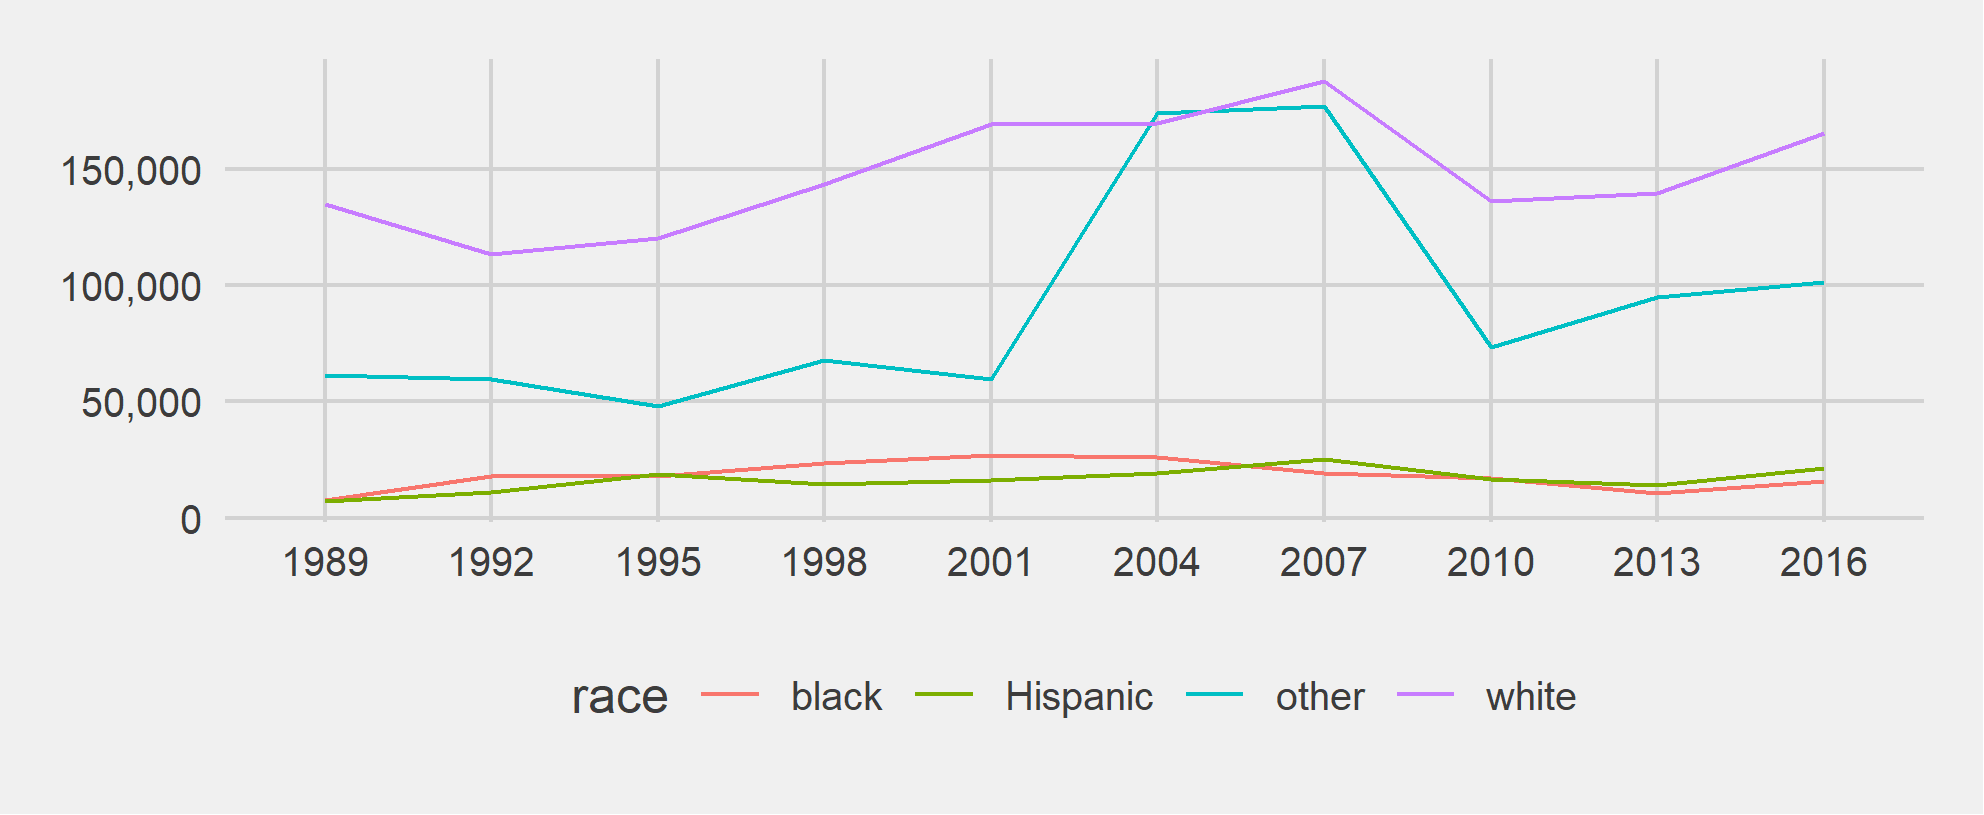
\includegraphics[width=\linewidth, height=5cm]{../median wealth finance_survey _by race .png}
	\end{subfigure}
	\begin{subfigure}{.49\textwidth}
	\centering
	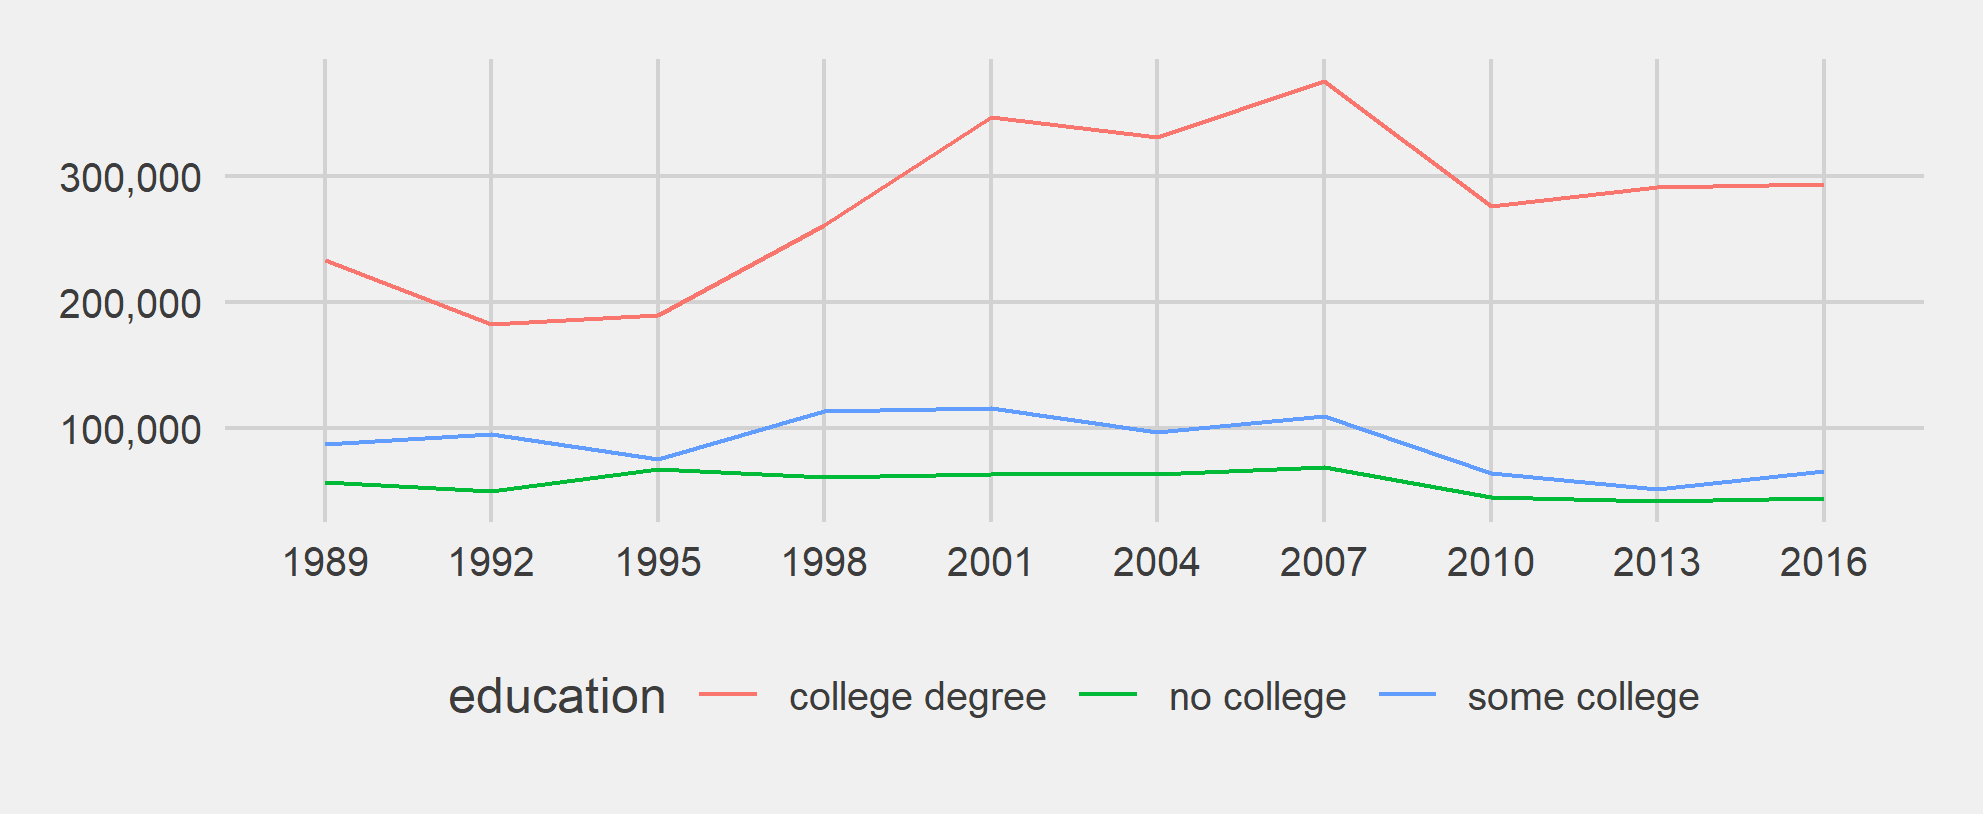
\includegraphics[width=\linewidth, height=5cm]{../median wealth finance_survey _by education .png}
	\end{subfigure}
	\begin{subfigure}{.49\textwidth}
	\centering
	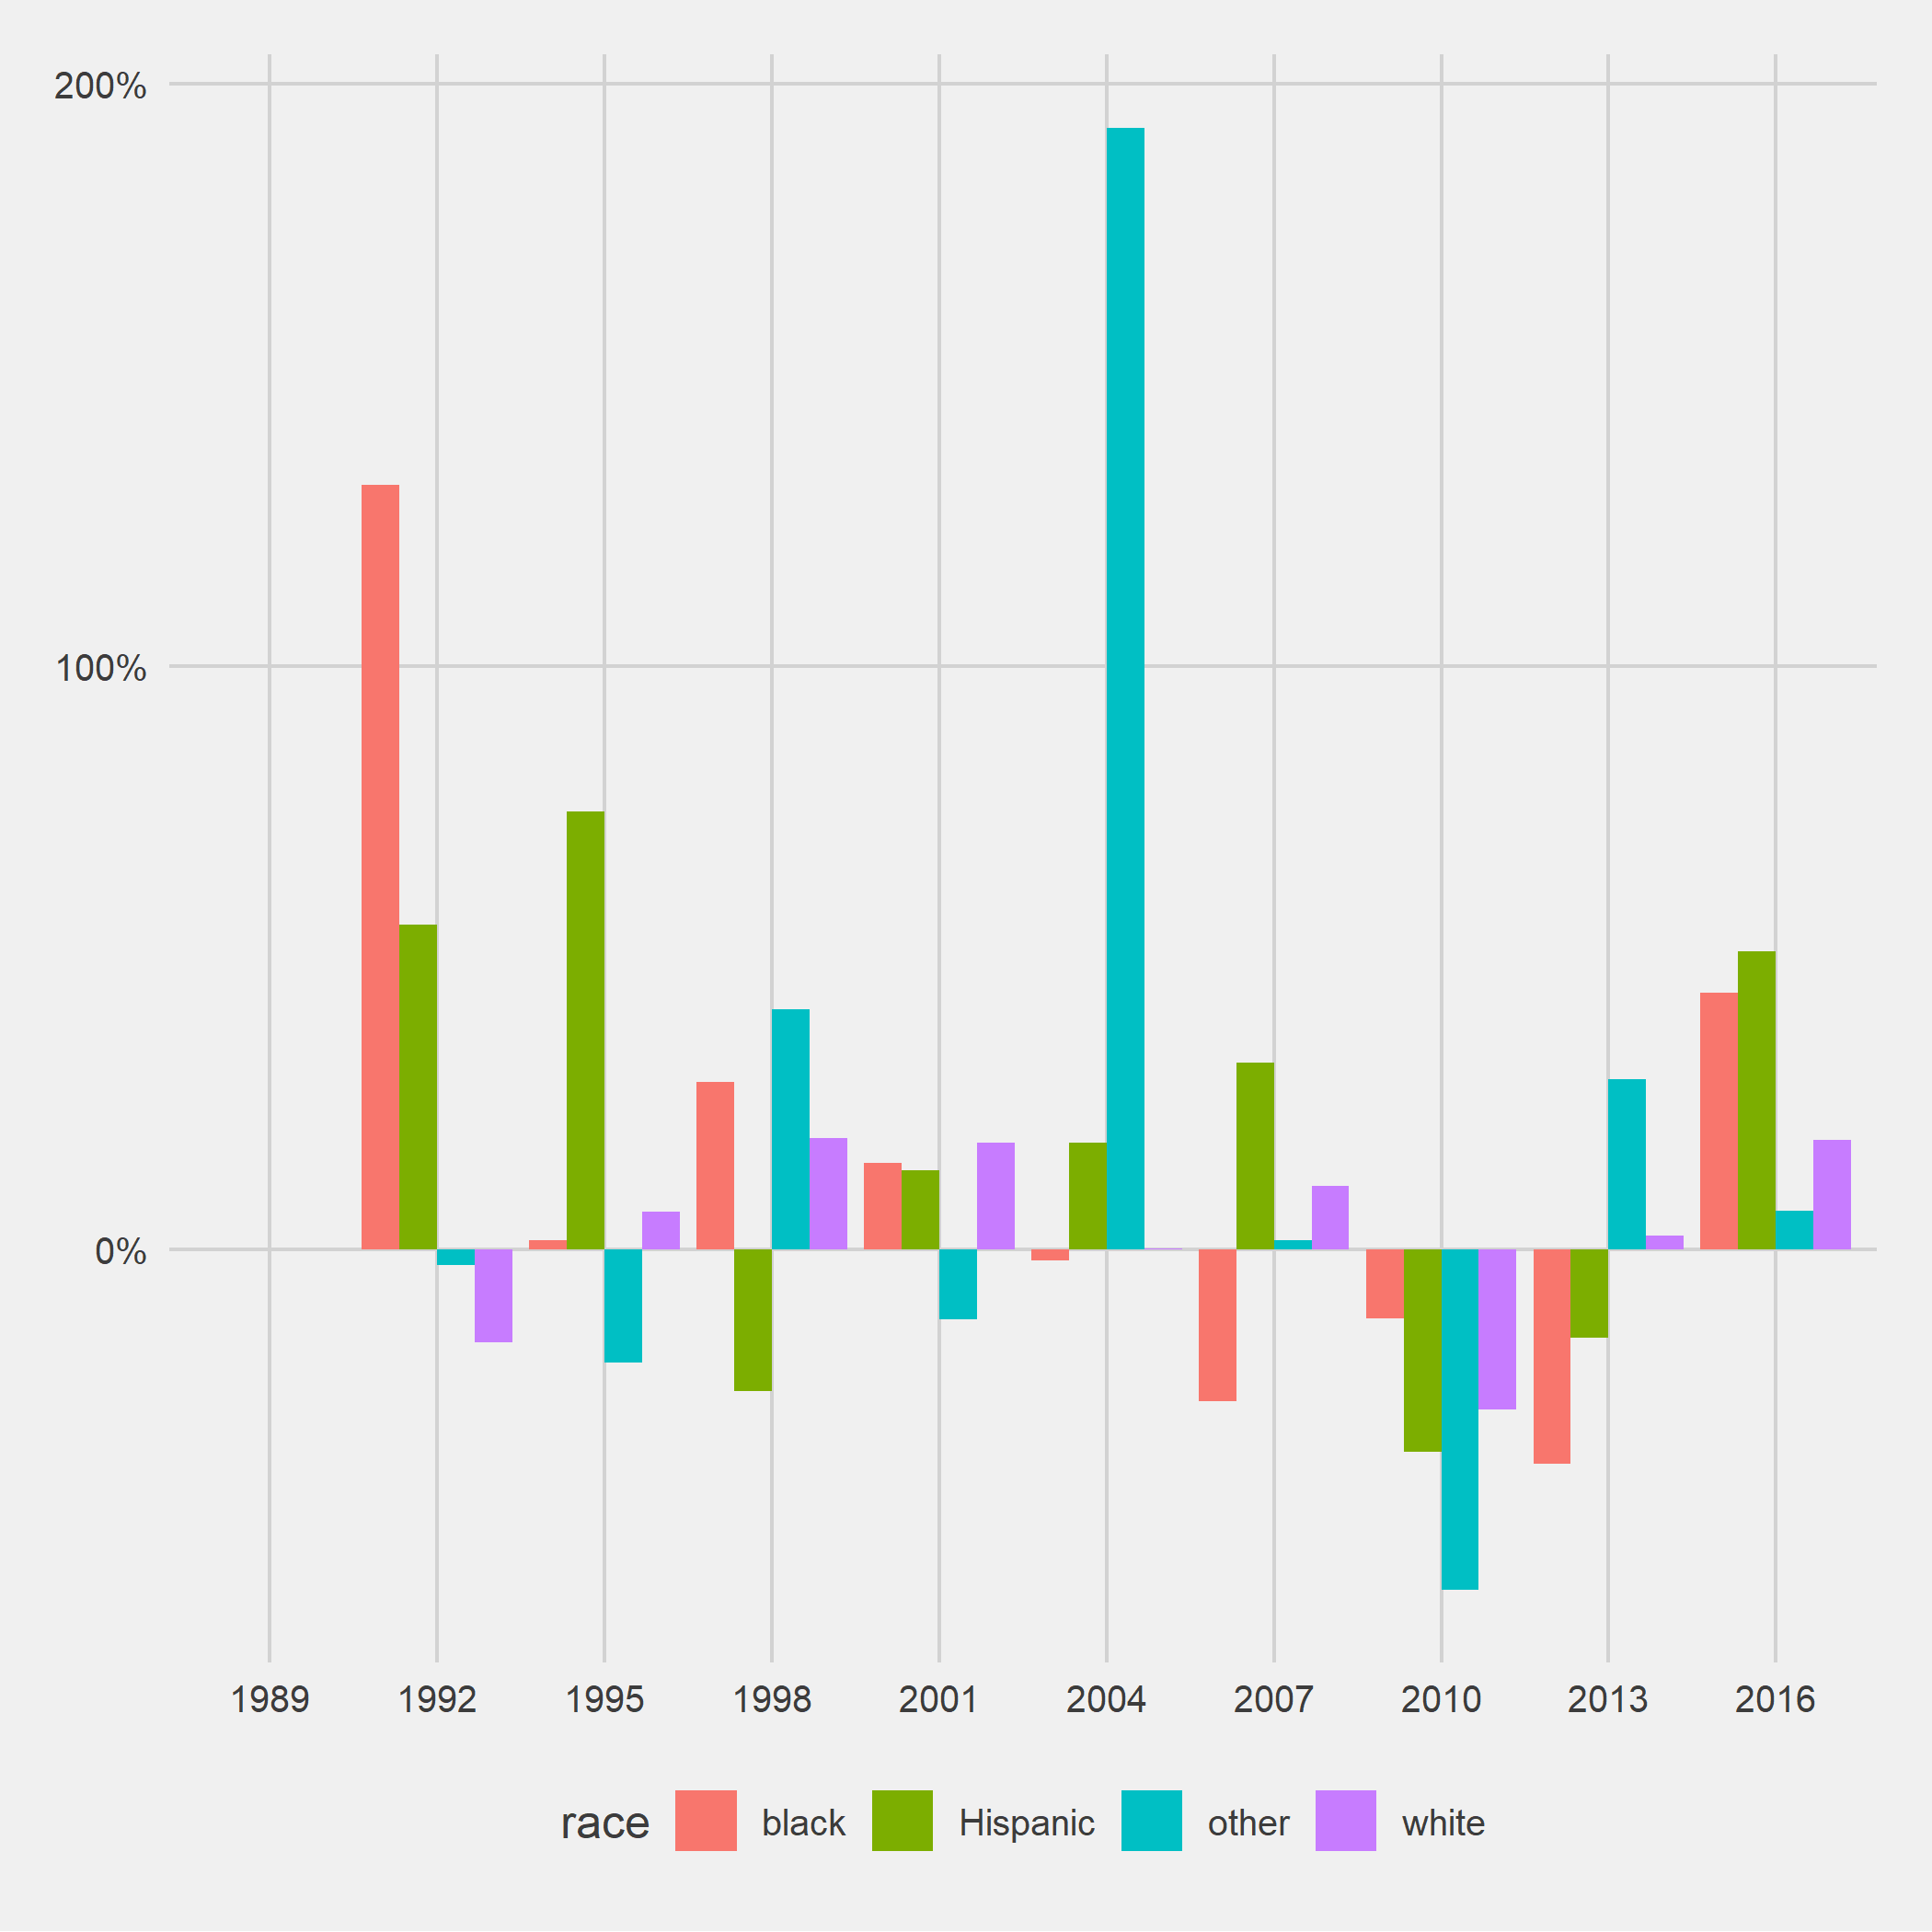
\includegraphics[width=\linewidth, height=5cm]{../change_median wealth finance_survey _by race .png}
	\end{subfigure}
	\begin{subfigure}{.49\textwidth}
	\centering
	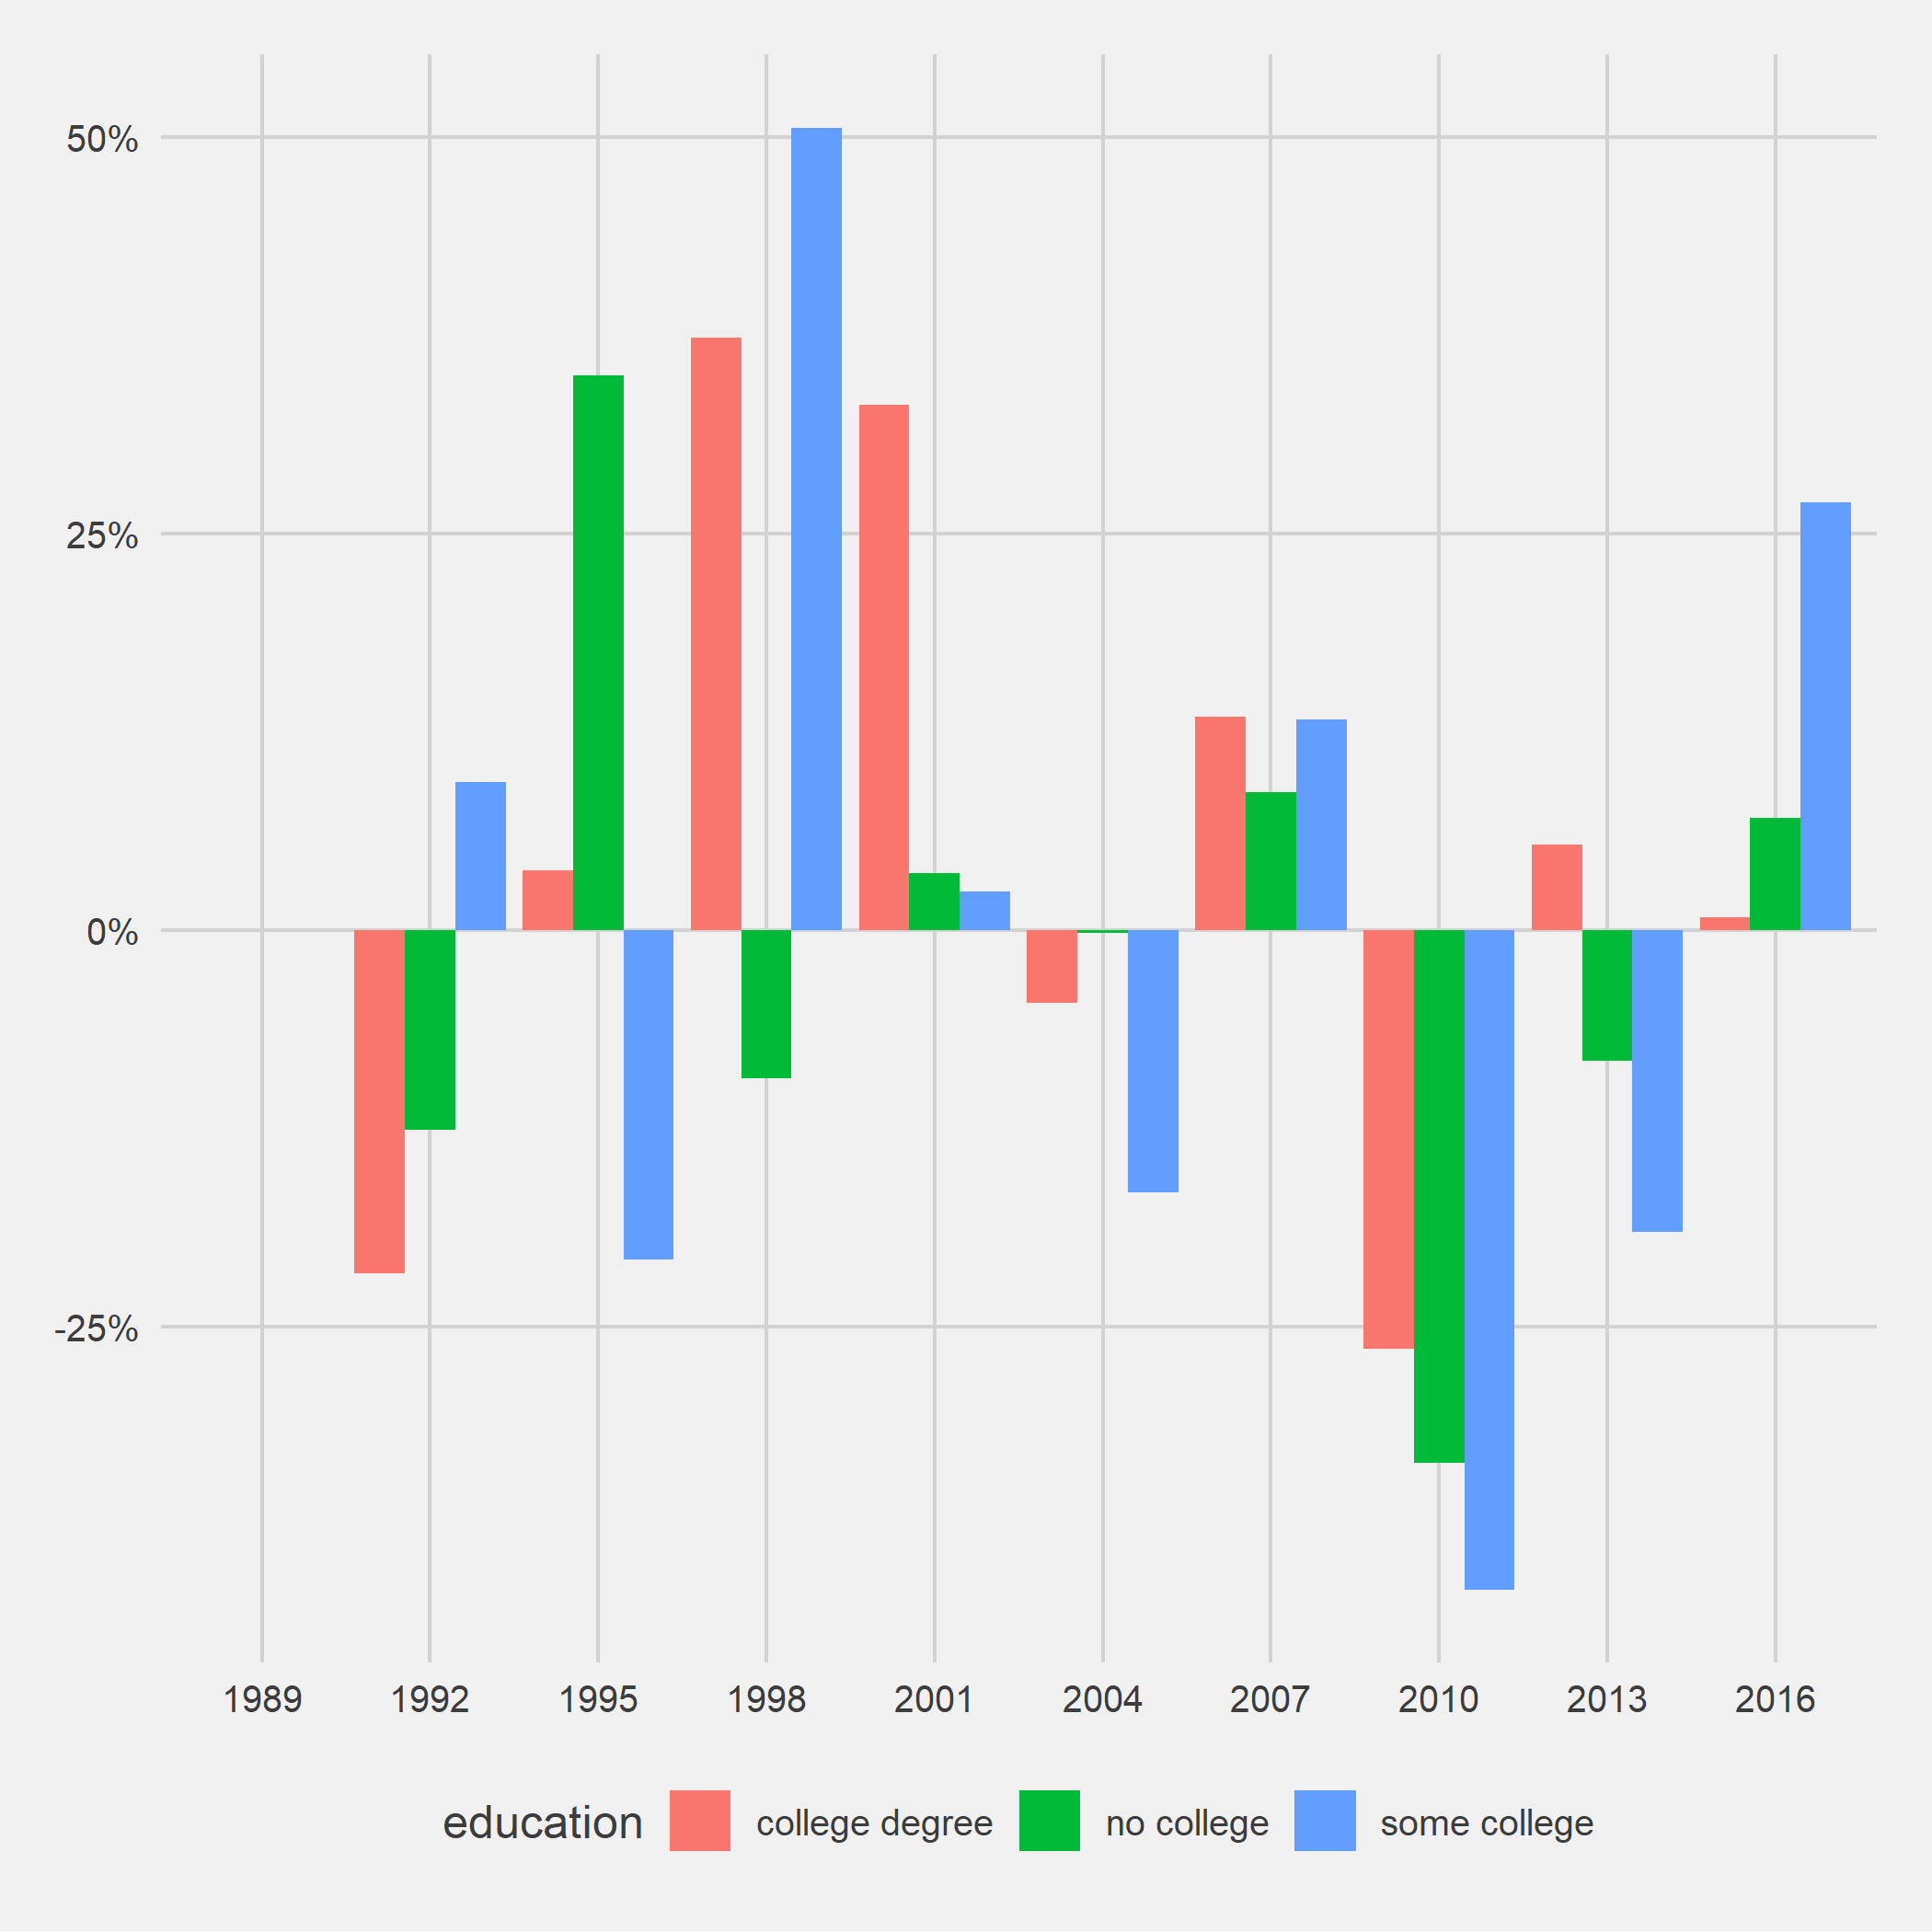
\includegraphics[width=\linewidth, height=5cm]{../change_median wealth finance_survey _by education .png}
	\end{subfigure}
	\caption{Median wealth in 2016 \$ over time by race and level of education}\label{fig:gen_trends}
\end{figure}

\subsection*{Question 2}
\textit{Repeat your analysis for just housing wealth for black and white households.} \\

Trends in median housing wealth for black and white households are depicted in Figure \ref{fig:bw_htrends}.
Again, one can observe stark level differences between white and black as well the college educated and less educated households. White housing wealth has evolved similar to regular wealth. One can see a large increase in wealth leading up to the financial crisis 2007 and a subsequent collapse. It is hard to draw any conclusions for the black population as their median remains at zero for the entire time-span of the sample. This indicates the high number of black households who do not have any housing wealth at all. \\
The trends by level of education take a similar from as for overall wealth. The college educated have more housing wealth to start with and see their wealth increase particularly strongly in the years prior to 2007. However, all education levels experience a strong collapse in their wealth after the financial crisis. In fact, in percentage terms this loss is least strong for the college educated.
\begin{figure}[h]
	\centering
	\begin{subfigure}{.49\textwidth}
		\centering
		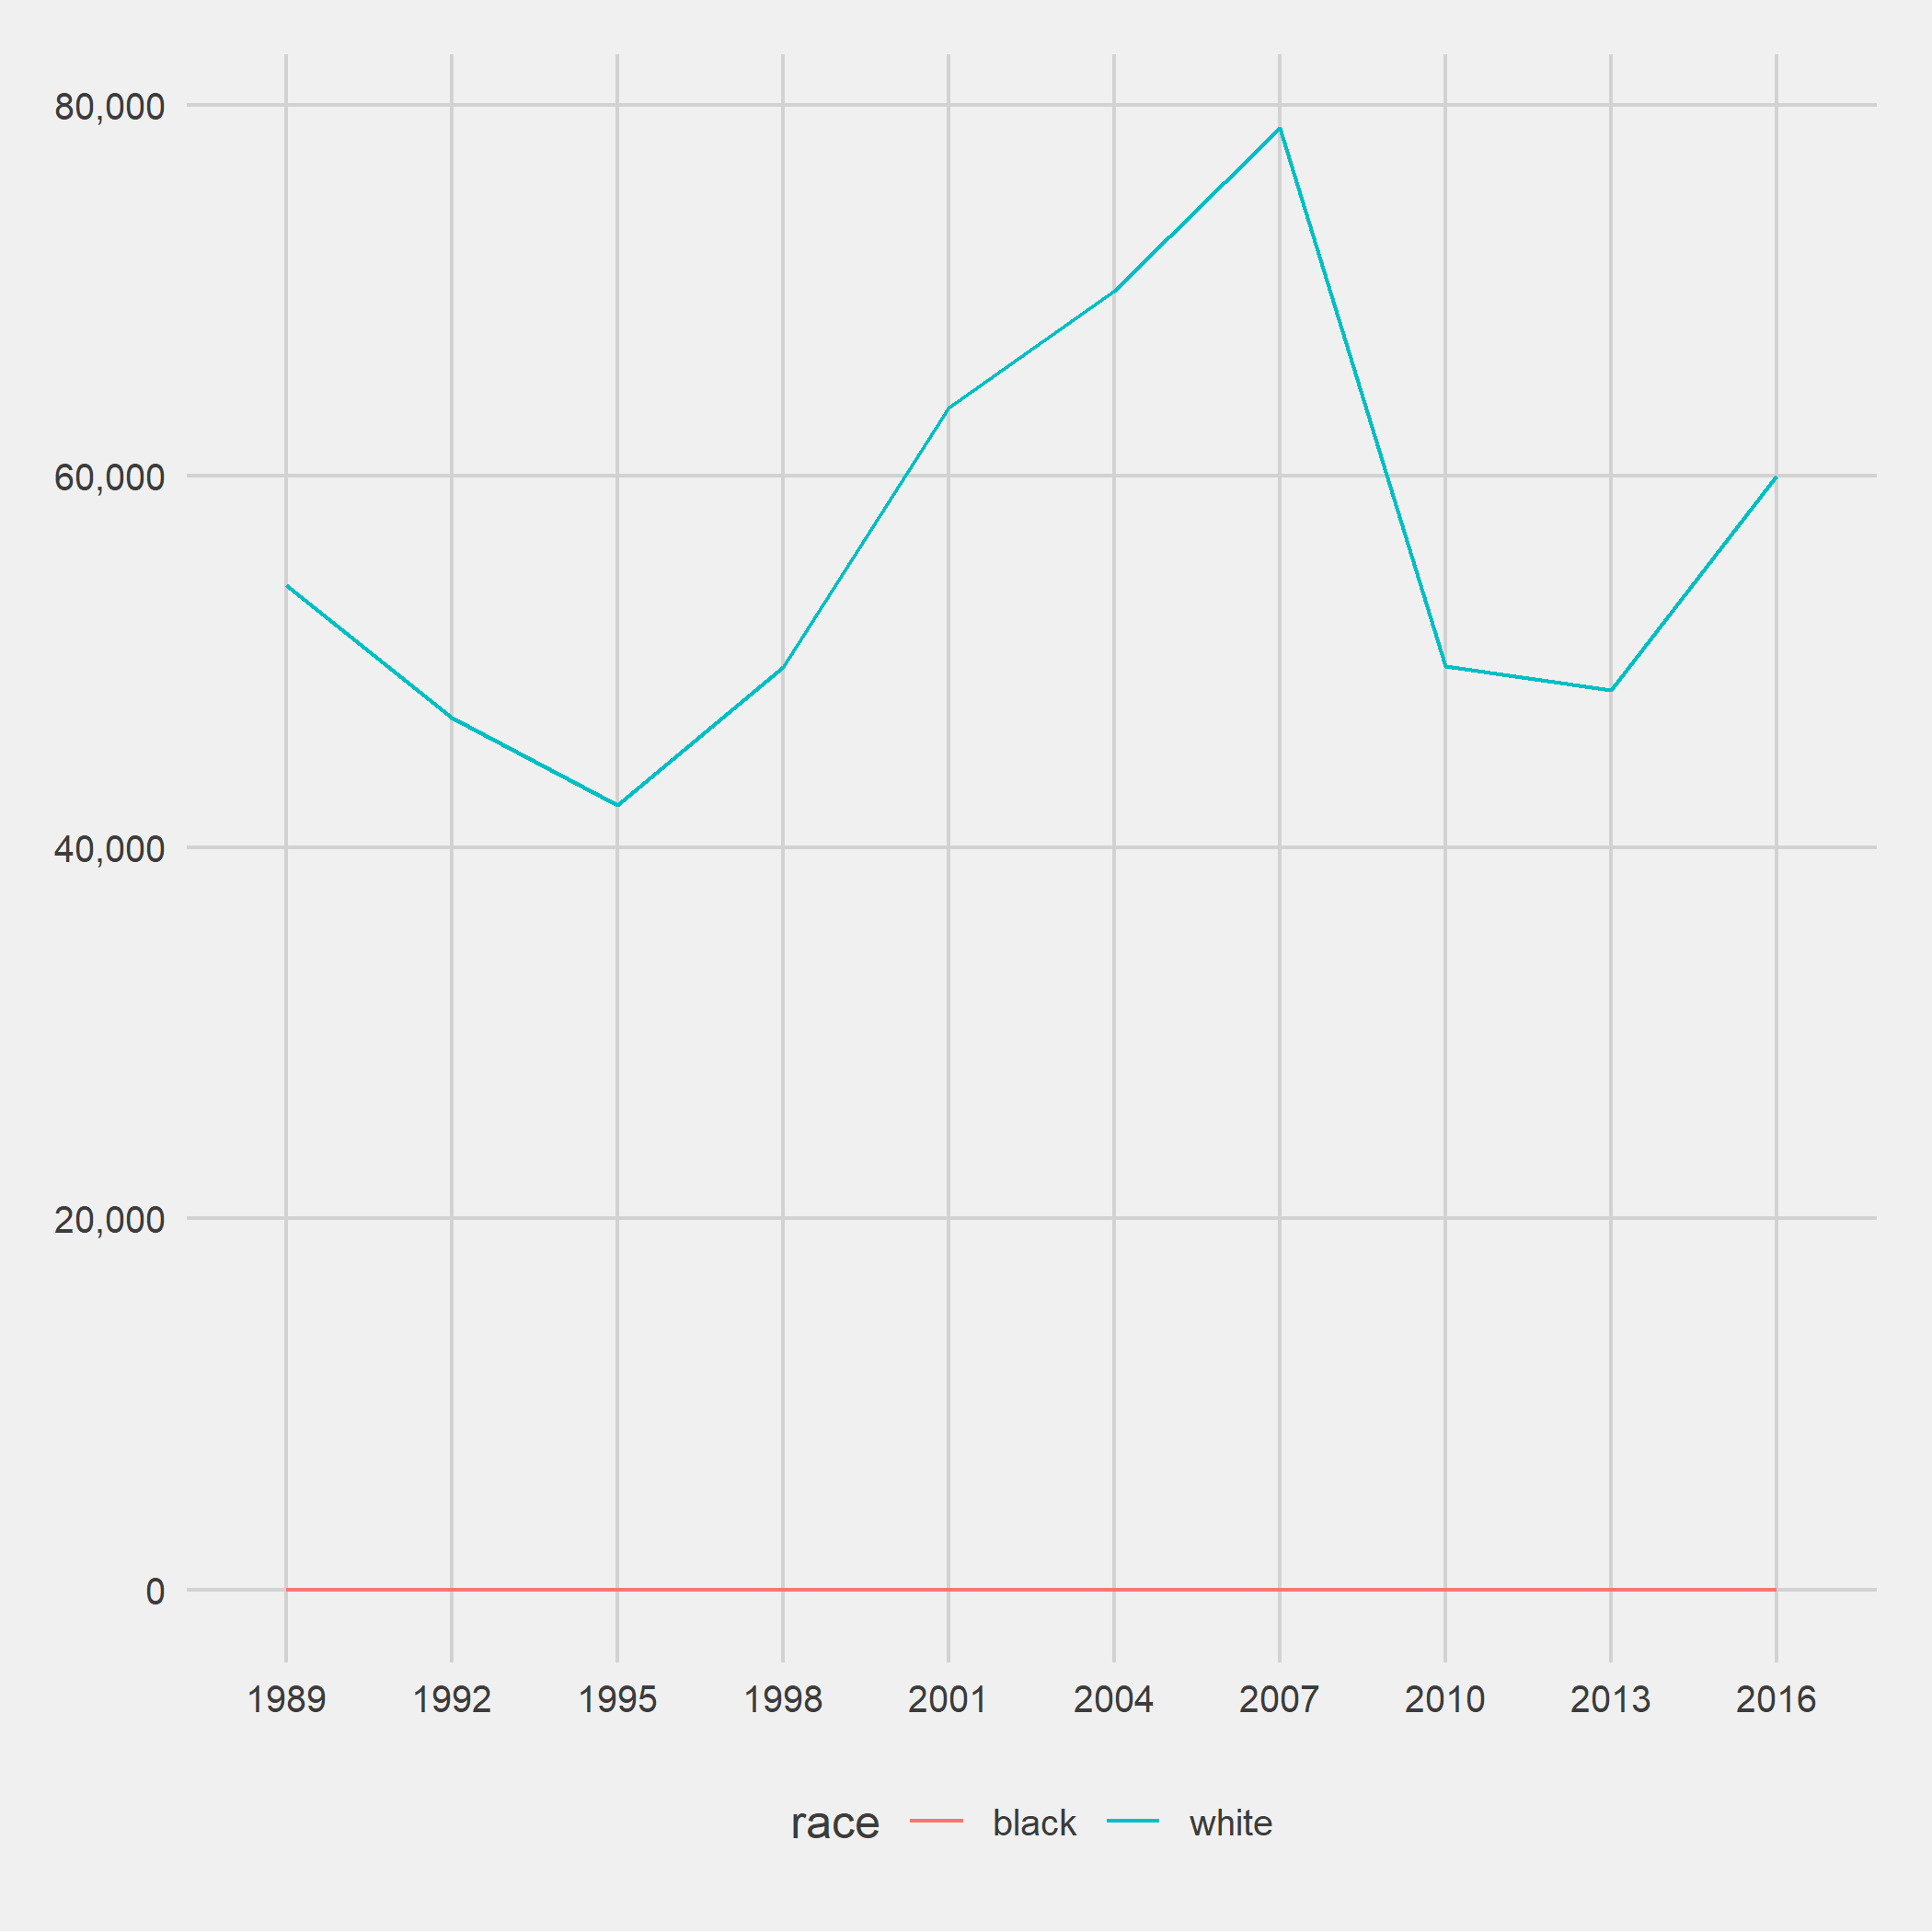
\includegraphics[width=\linewidth, height=5cm]{../median hwealth finance_survey_bw _by race .png}
	\end{subfigure}
	\begin{subfigure}{.49\textwidth}
		\centering
		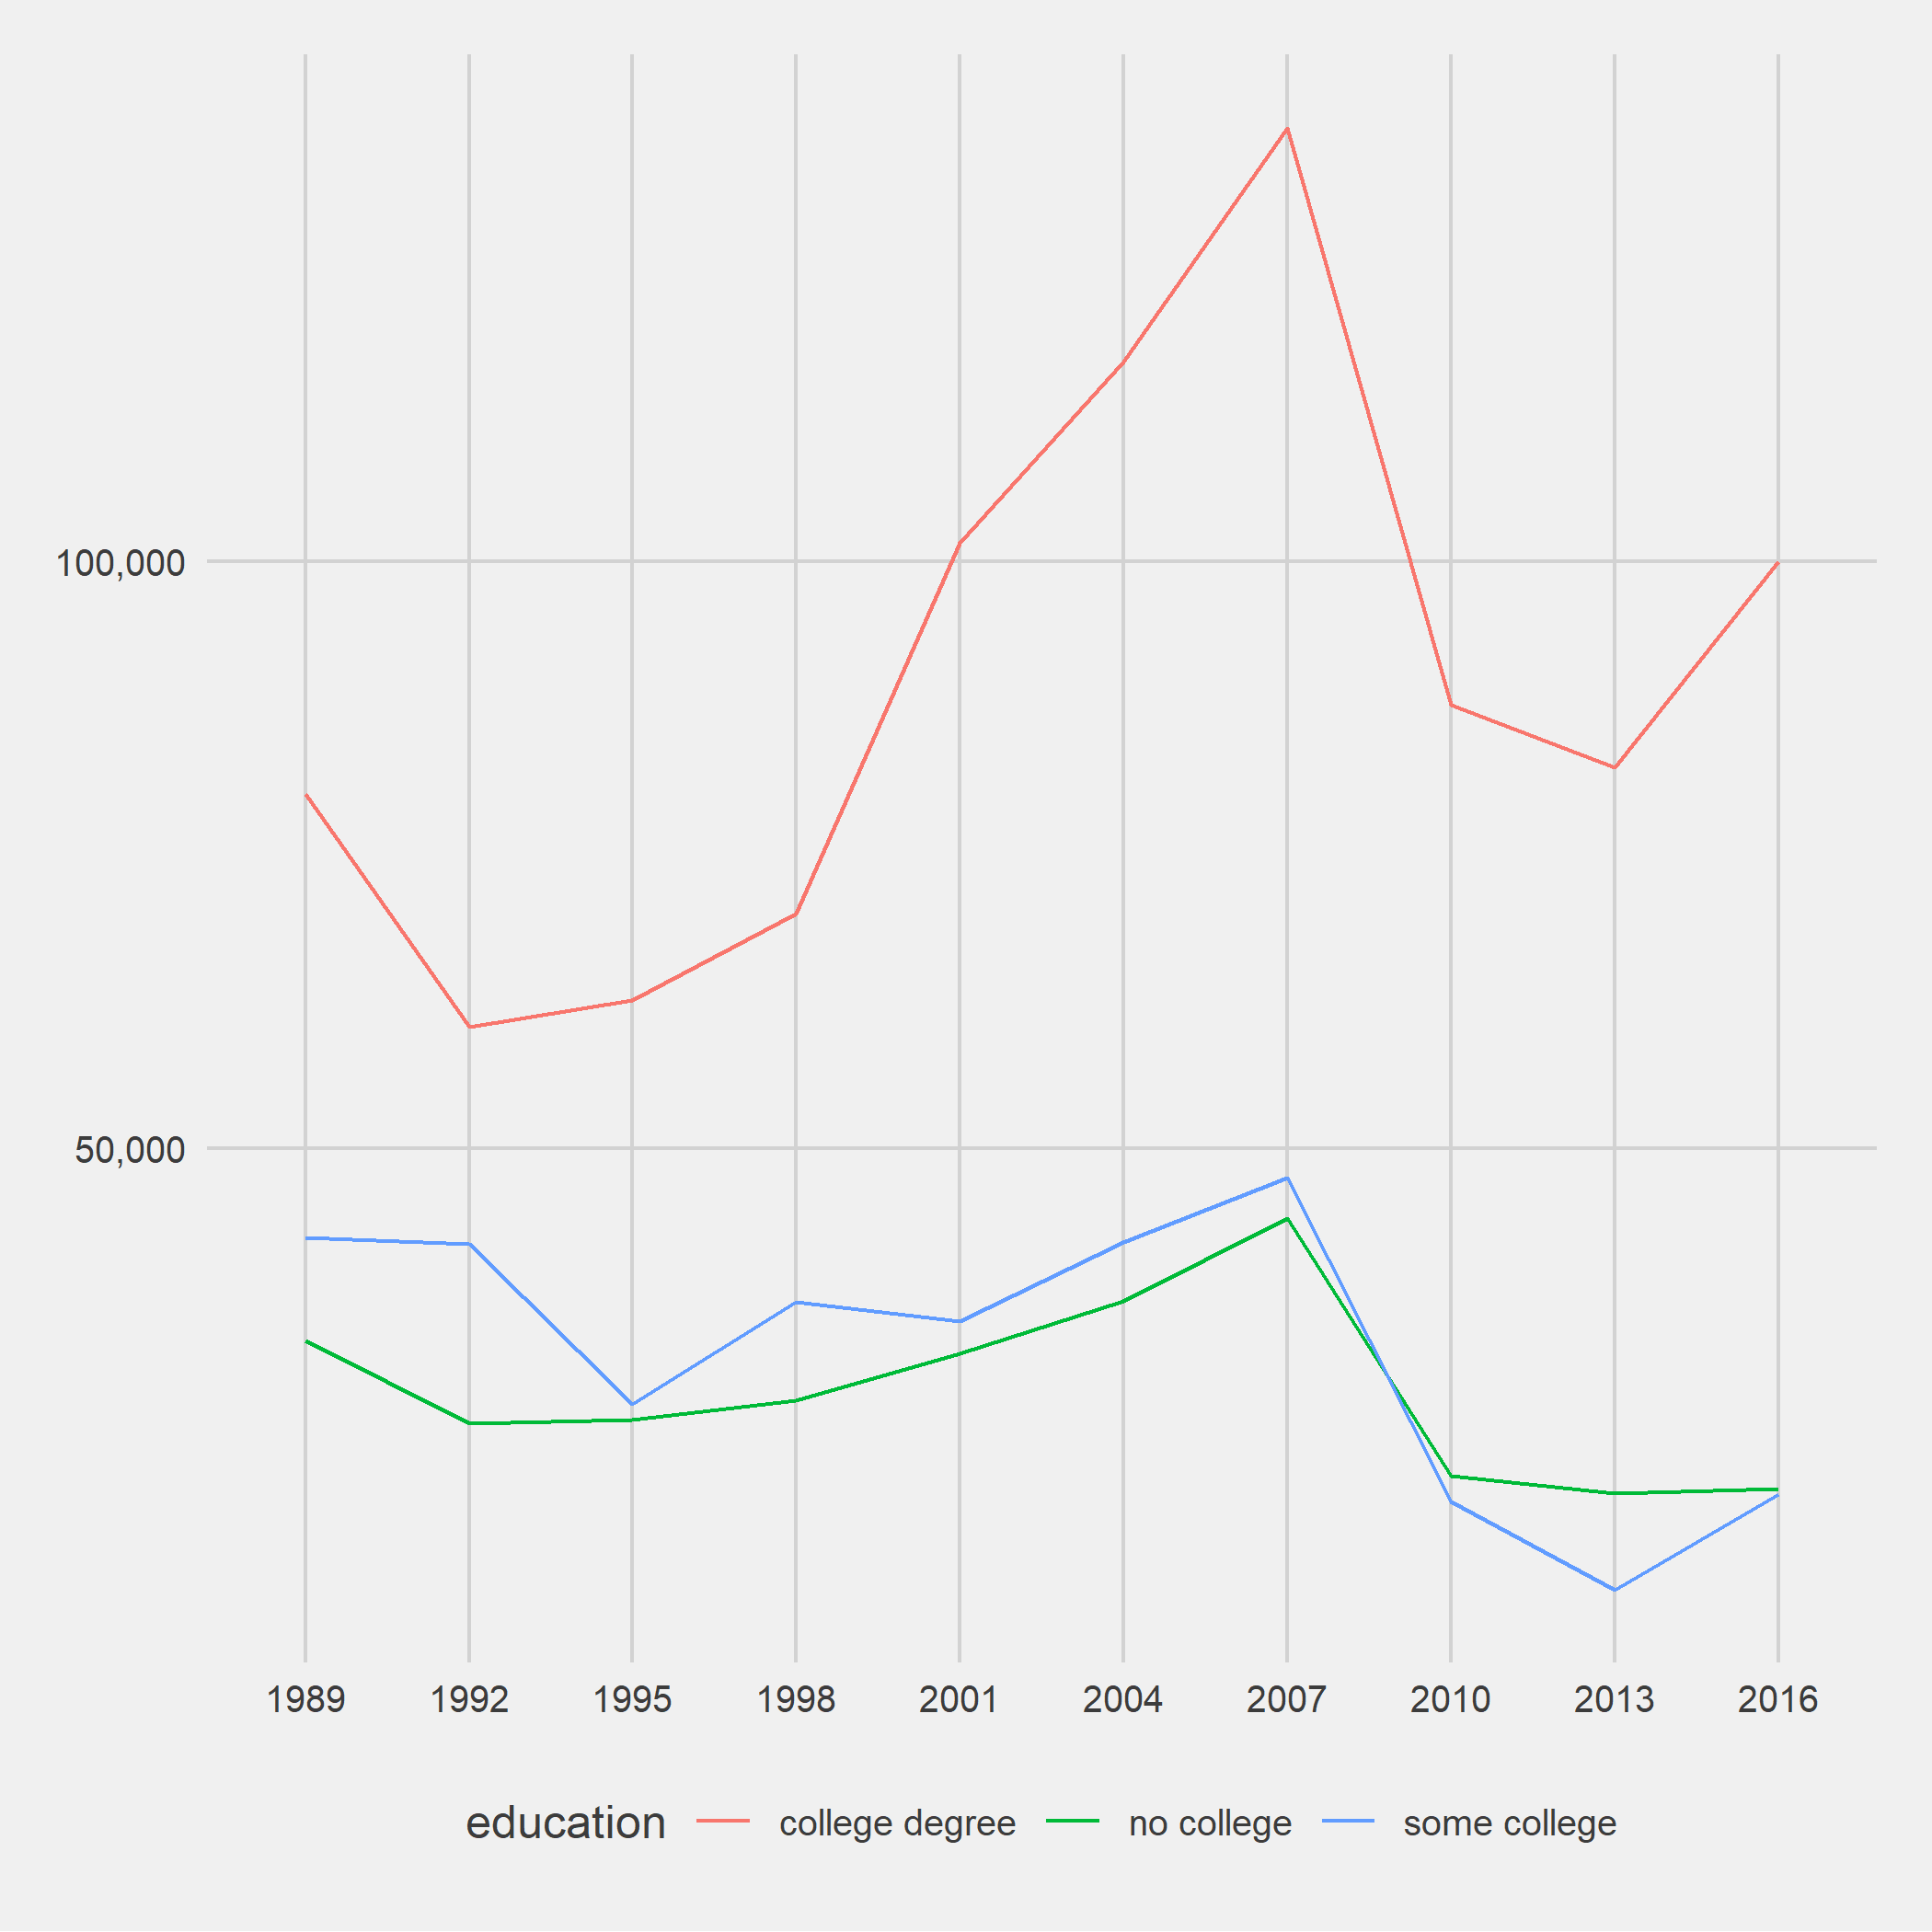
\includegraphics[width=\linewidth, height=5cm]{../median hwealth finance_survey_bw _by education .png}
	\end{subfigure}
	\begin{subfigure}{.49\textwidth}
	\centering
	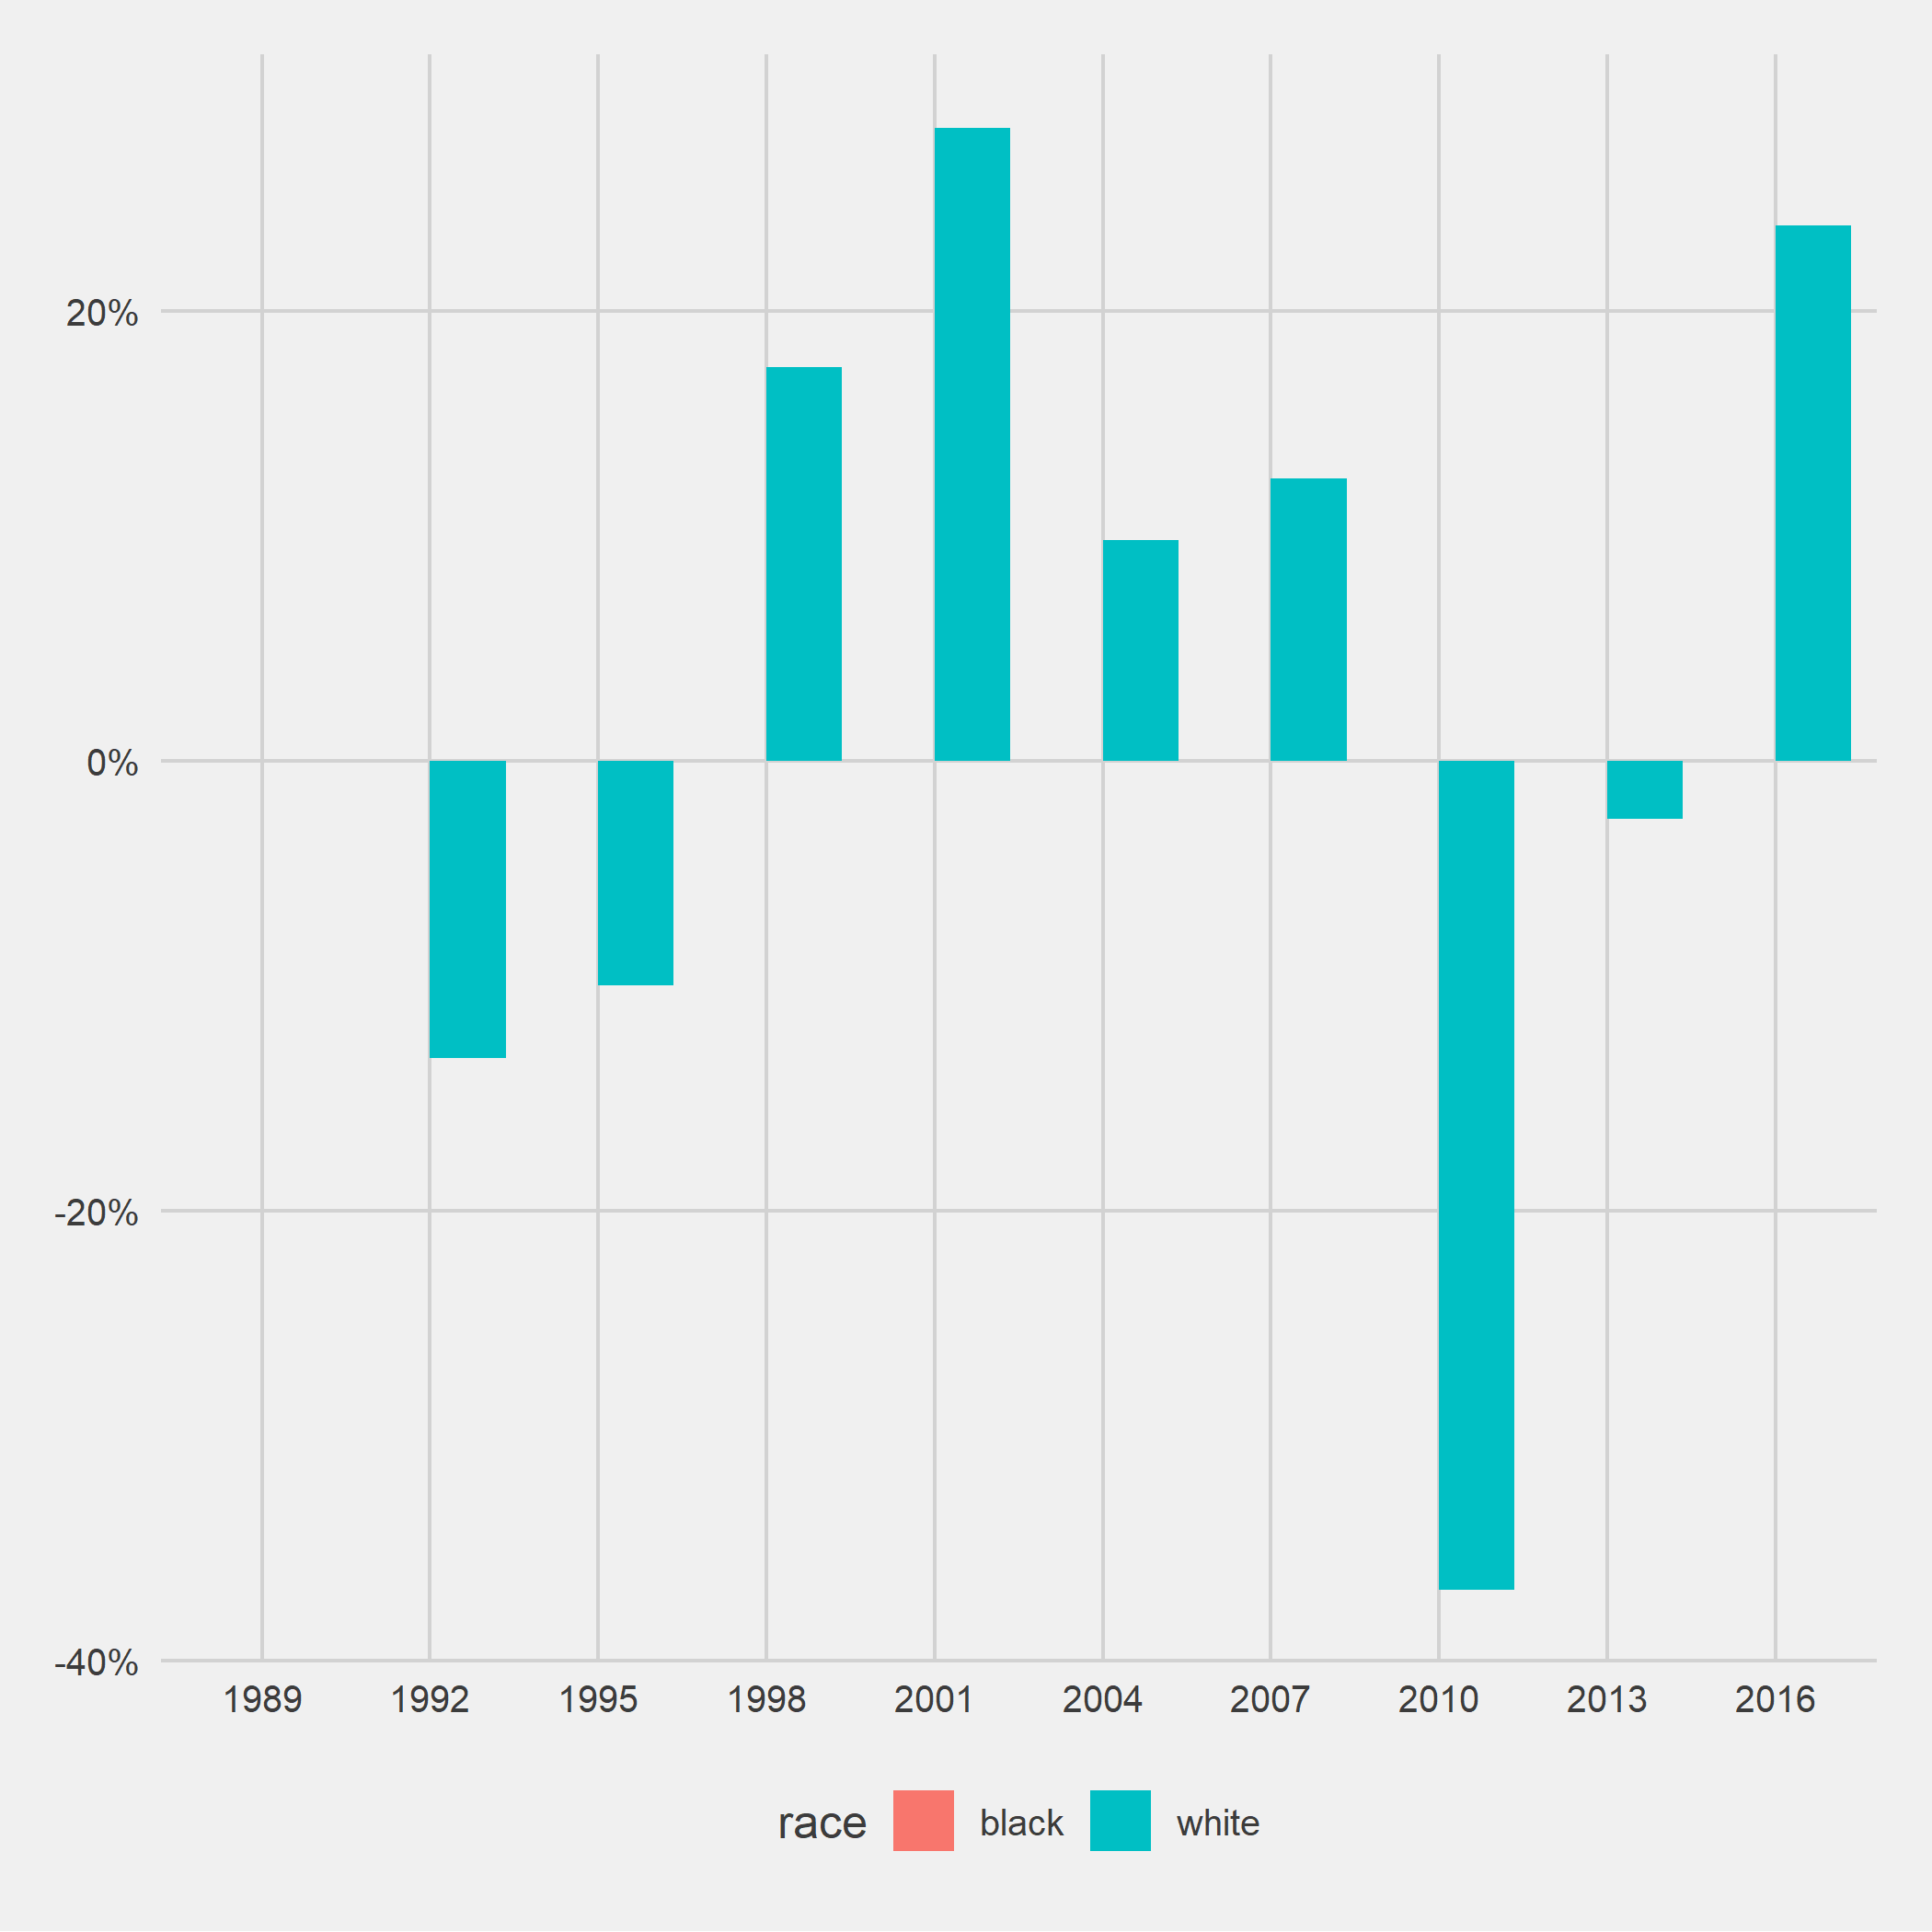
\includegraphics[width=\linewidth, height=5cm]{../change_median hwealth finance_survey_bw _by race .png}
	\end{subfigure}
	\begin{subfigure}{.49\textwidth}
	\centering
	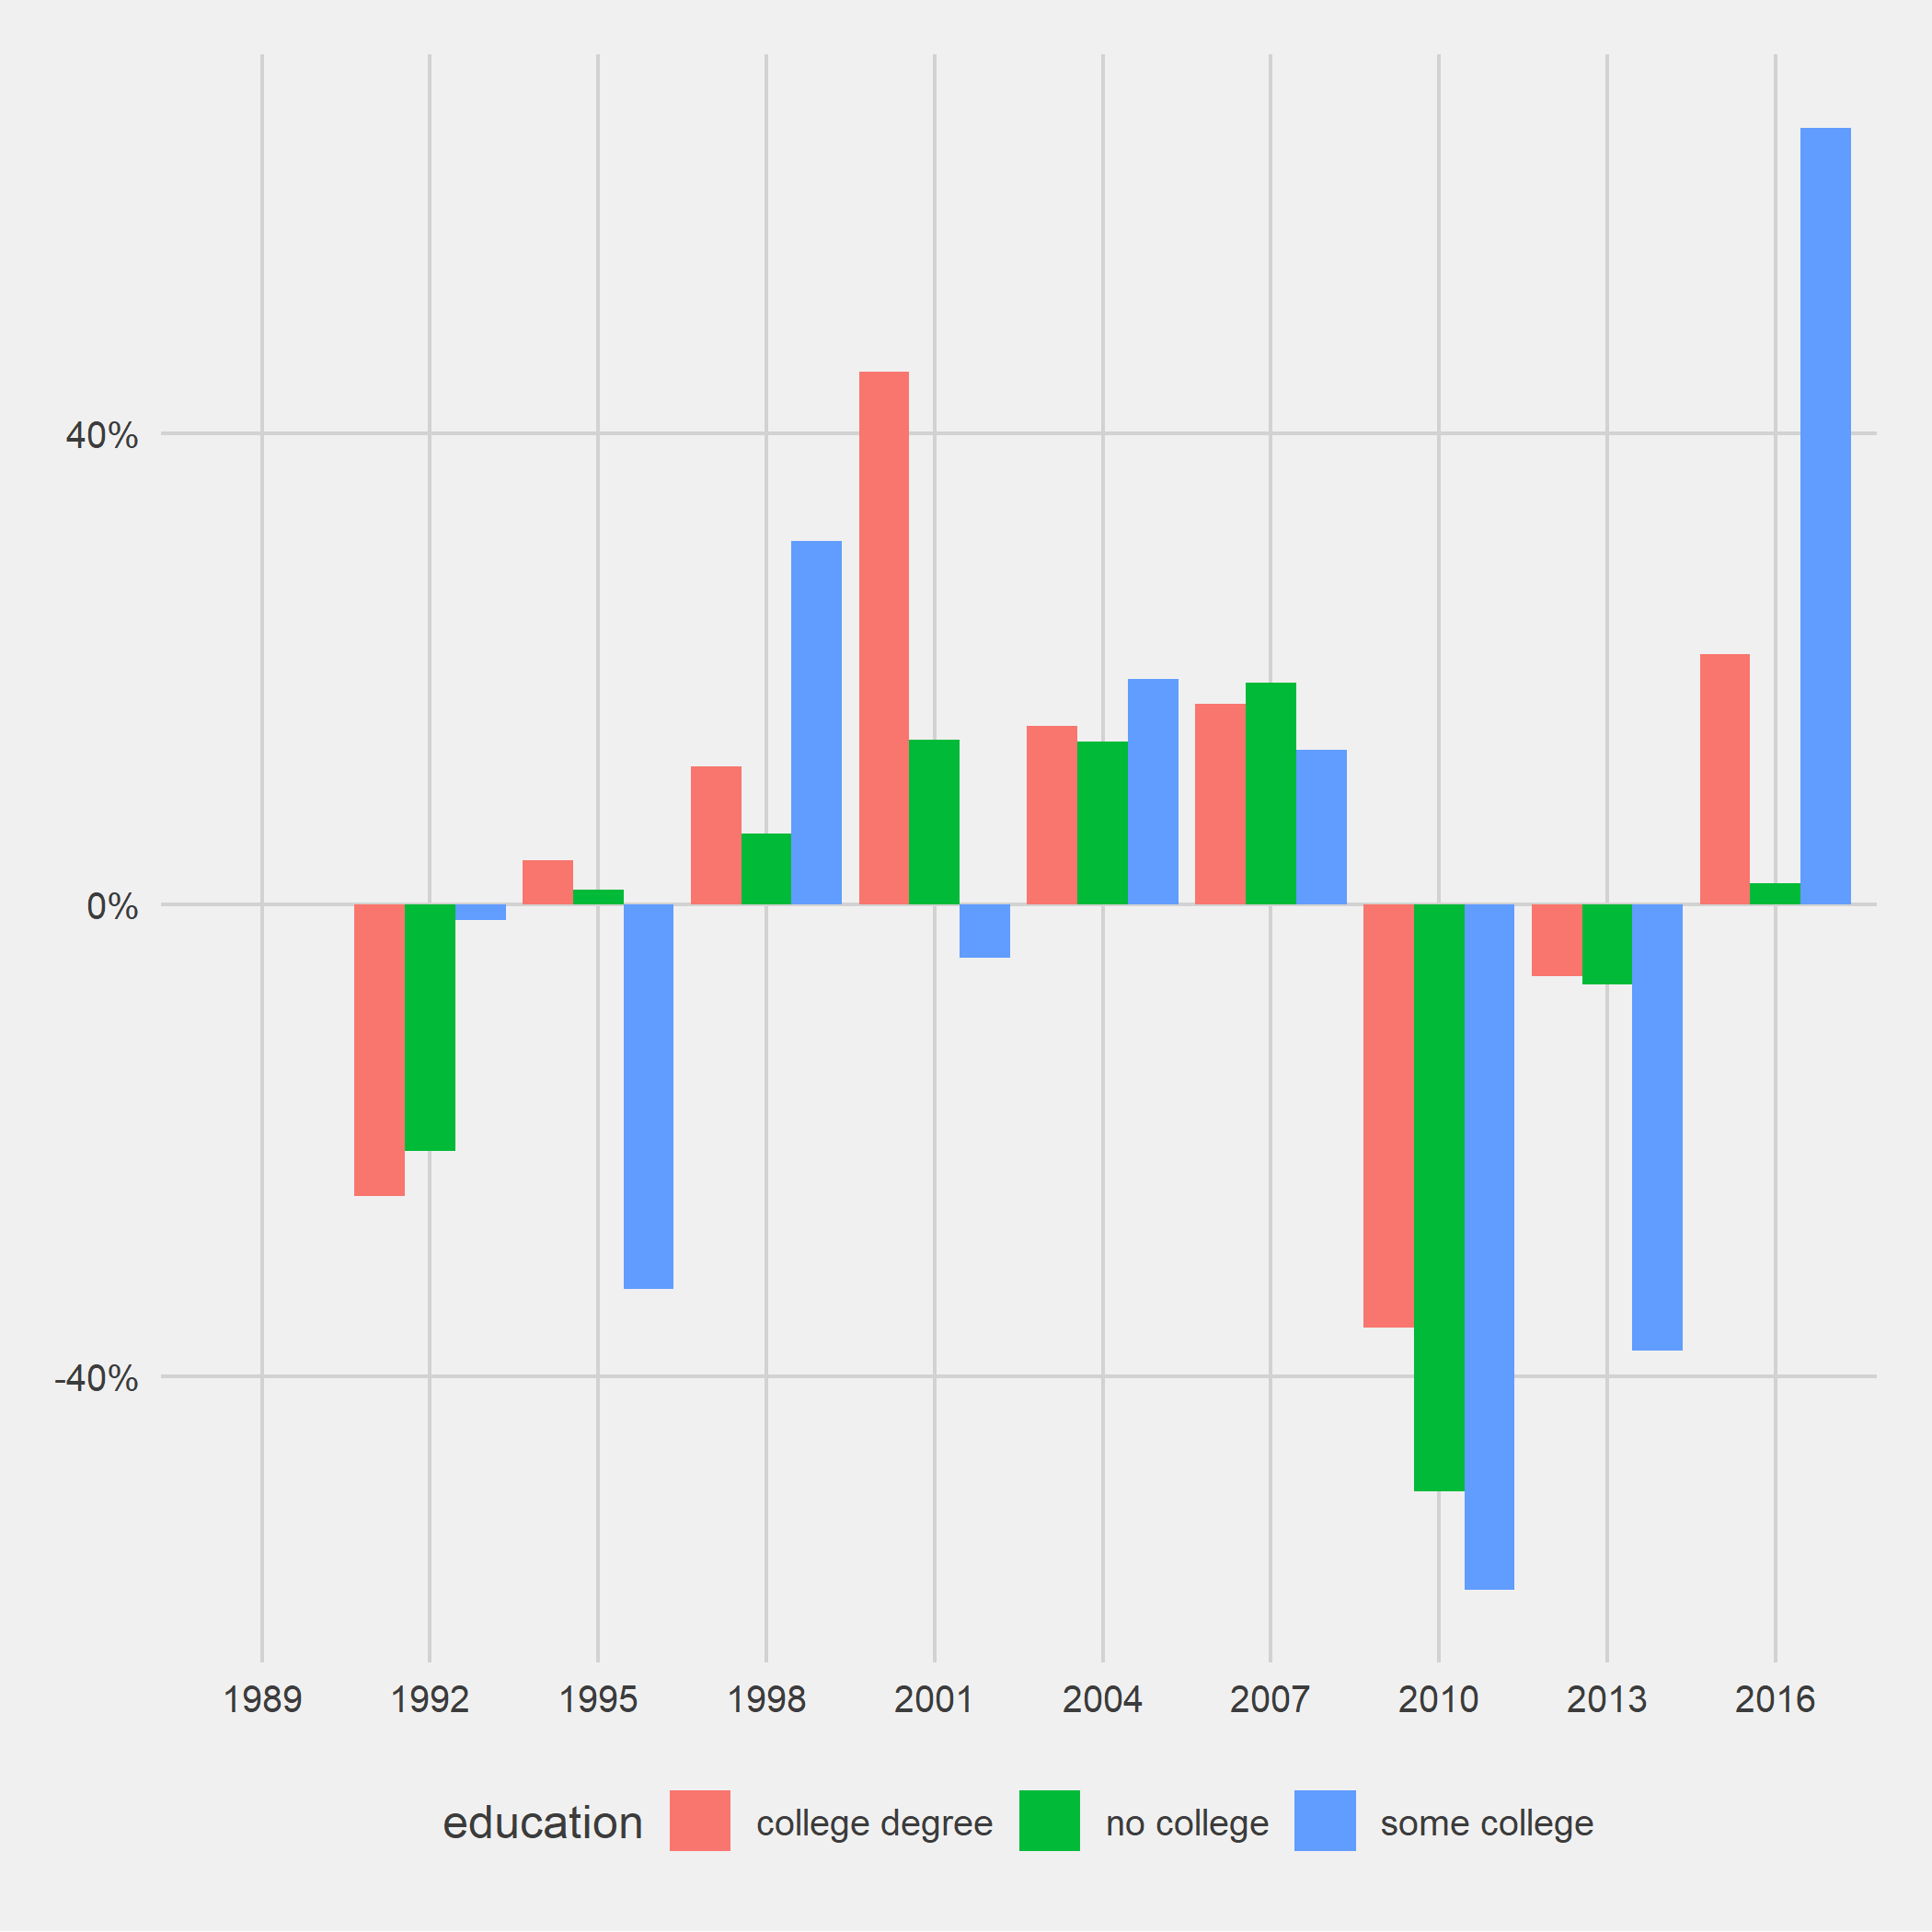
\includegraphics[width=\linewidth, height=5cm]{../change_median hwealth finance_survey_bw _by education .png}
	\end{subfigure}
	\caption{Median wealth in 2016 \$ over time by race and level of education}\label{fig:bw_htrends}
\end{figure}

\subsection*{Question 3}
\textit{Many households are not homeowners and so your analysis for the prior question includes many zeros
	for housing wealth. Let’s dig deeper by focusing just on homeowners age 25 or older. Please summarize
	trends in for black and white households for both housing and non-housing wealth. Which group had
	the largest loss in housing wealth, where 2007 is defined as the base period? Please answer this question
	both in dollar terms and in proportional terms.} \\

Figure \ref{fig:bw25_htrends} depicts trends in housing and non-housing wealth for black and white homeowners age 25 or older. Overall, trends for black and white households are similar. White housing wealth evolves comparable to what I already observed in Figure \ref{fig:bw_htrends}. Limiting the analysis to actual homeowners enables one to also observe trends in the black population. Both groups see their housing wealth grow significantly in the years before 2007 and collapse afterwards. Further, they experience a strong recovery after 2013. \\
In terms of non-housing wealth the trends are slightly shifted. Both black and white households experience strong growth in the nineties but after that the trends diverge. White non-housing wealth falls until after the financial crisis and starts recovering after 2010 whereas black wealth initially declines as well but then rebounds very strongly up to 2007 after it declines again. \\
Table 1 answers the question of which group had the largest loss in housing wealth after 2007. I show both the relative and absolute losses for three and nine years after 2007. It is interesting to distinguish these as groups who experienced large losses after 2007 also recovered very strongly after 2013. Clearly, both in absolute and relative terms, white households have experienced the largest loss, however, the difference between black and white households shrinks if one looks at proportional losses rather than absolute losses.
\begin{figure}[h]
	\centering
	\begin{subfigure}{.49\textwidth}
		\centering
		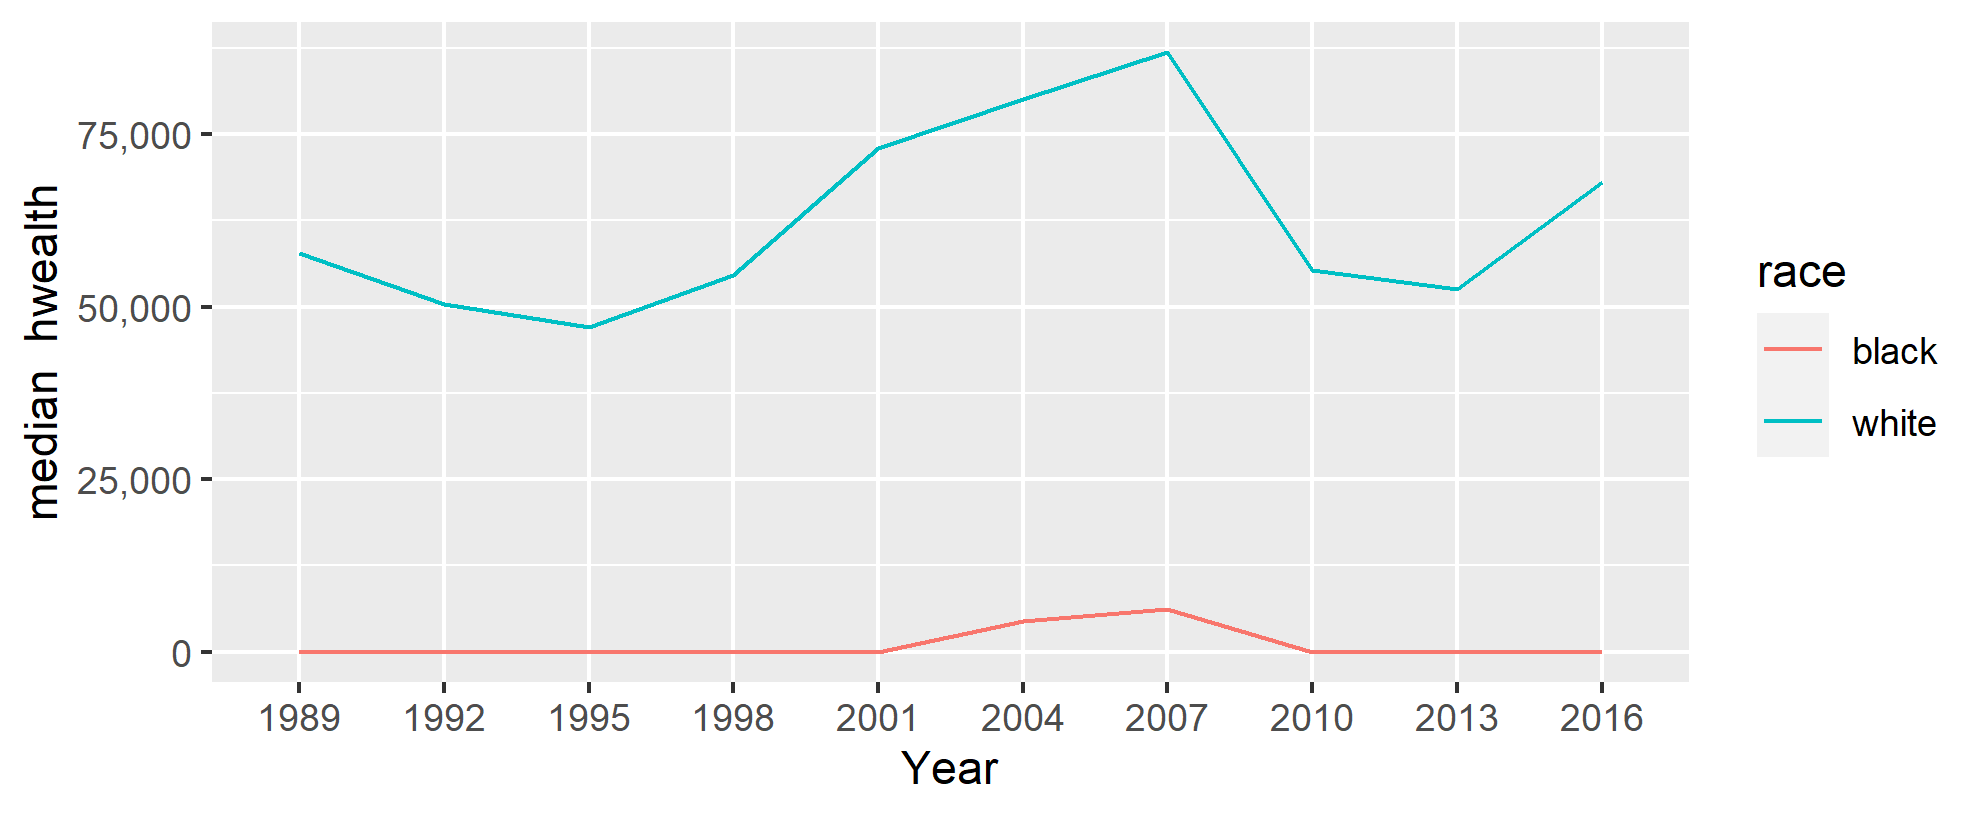
\includegraphics[width=\linewidth, height=5cm]{../median hwealth finance_survey_bw_25 _by race .png}
	\end{subfigure}
	\begin{subfigure}{.49\textwidth}
		\centering
		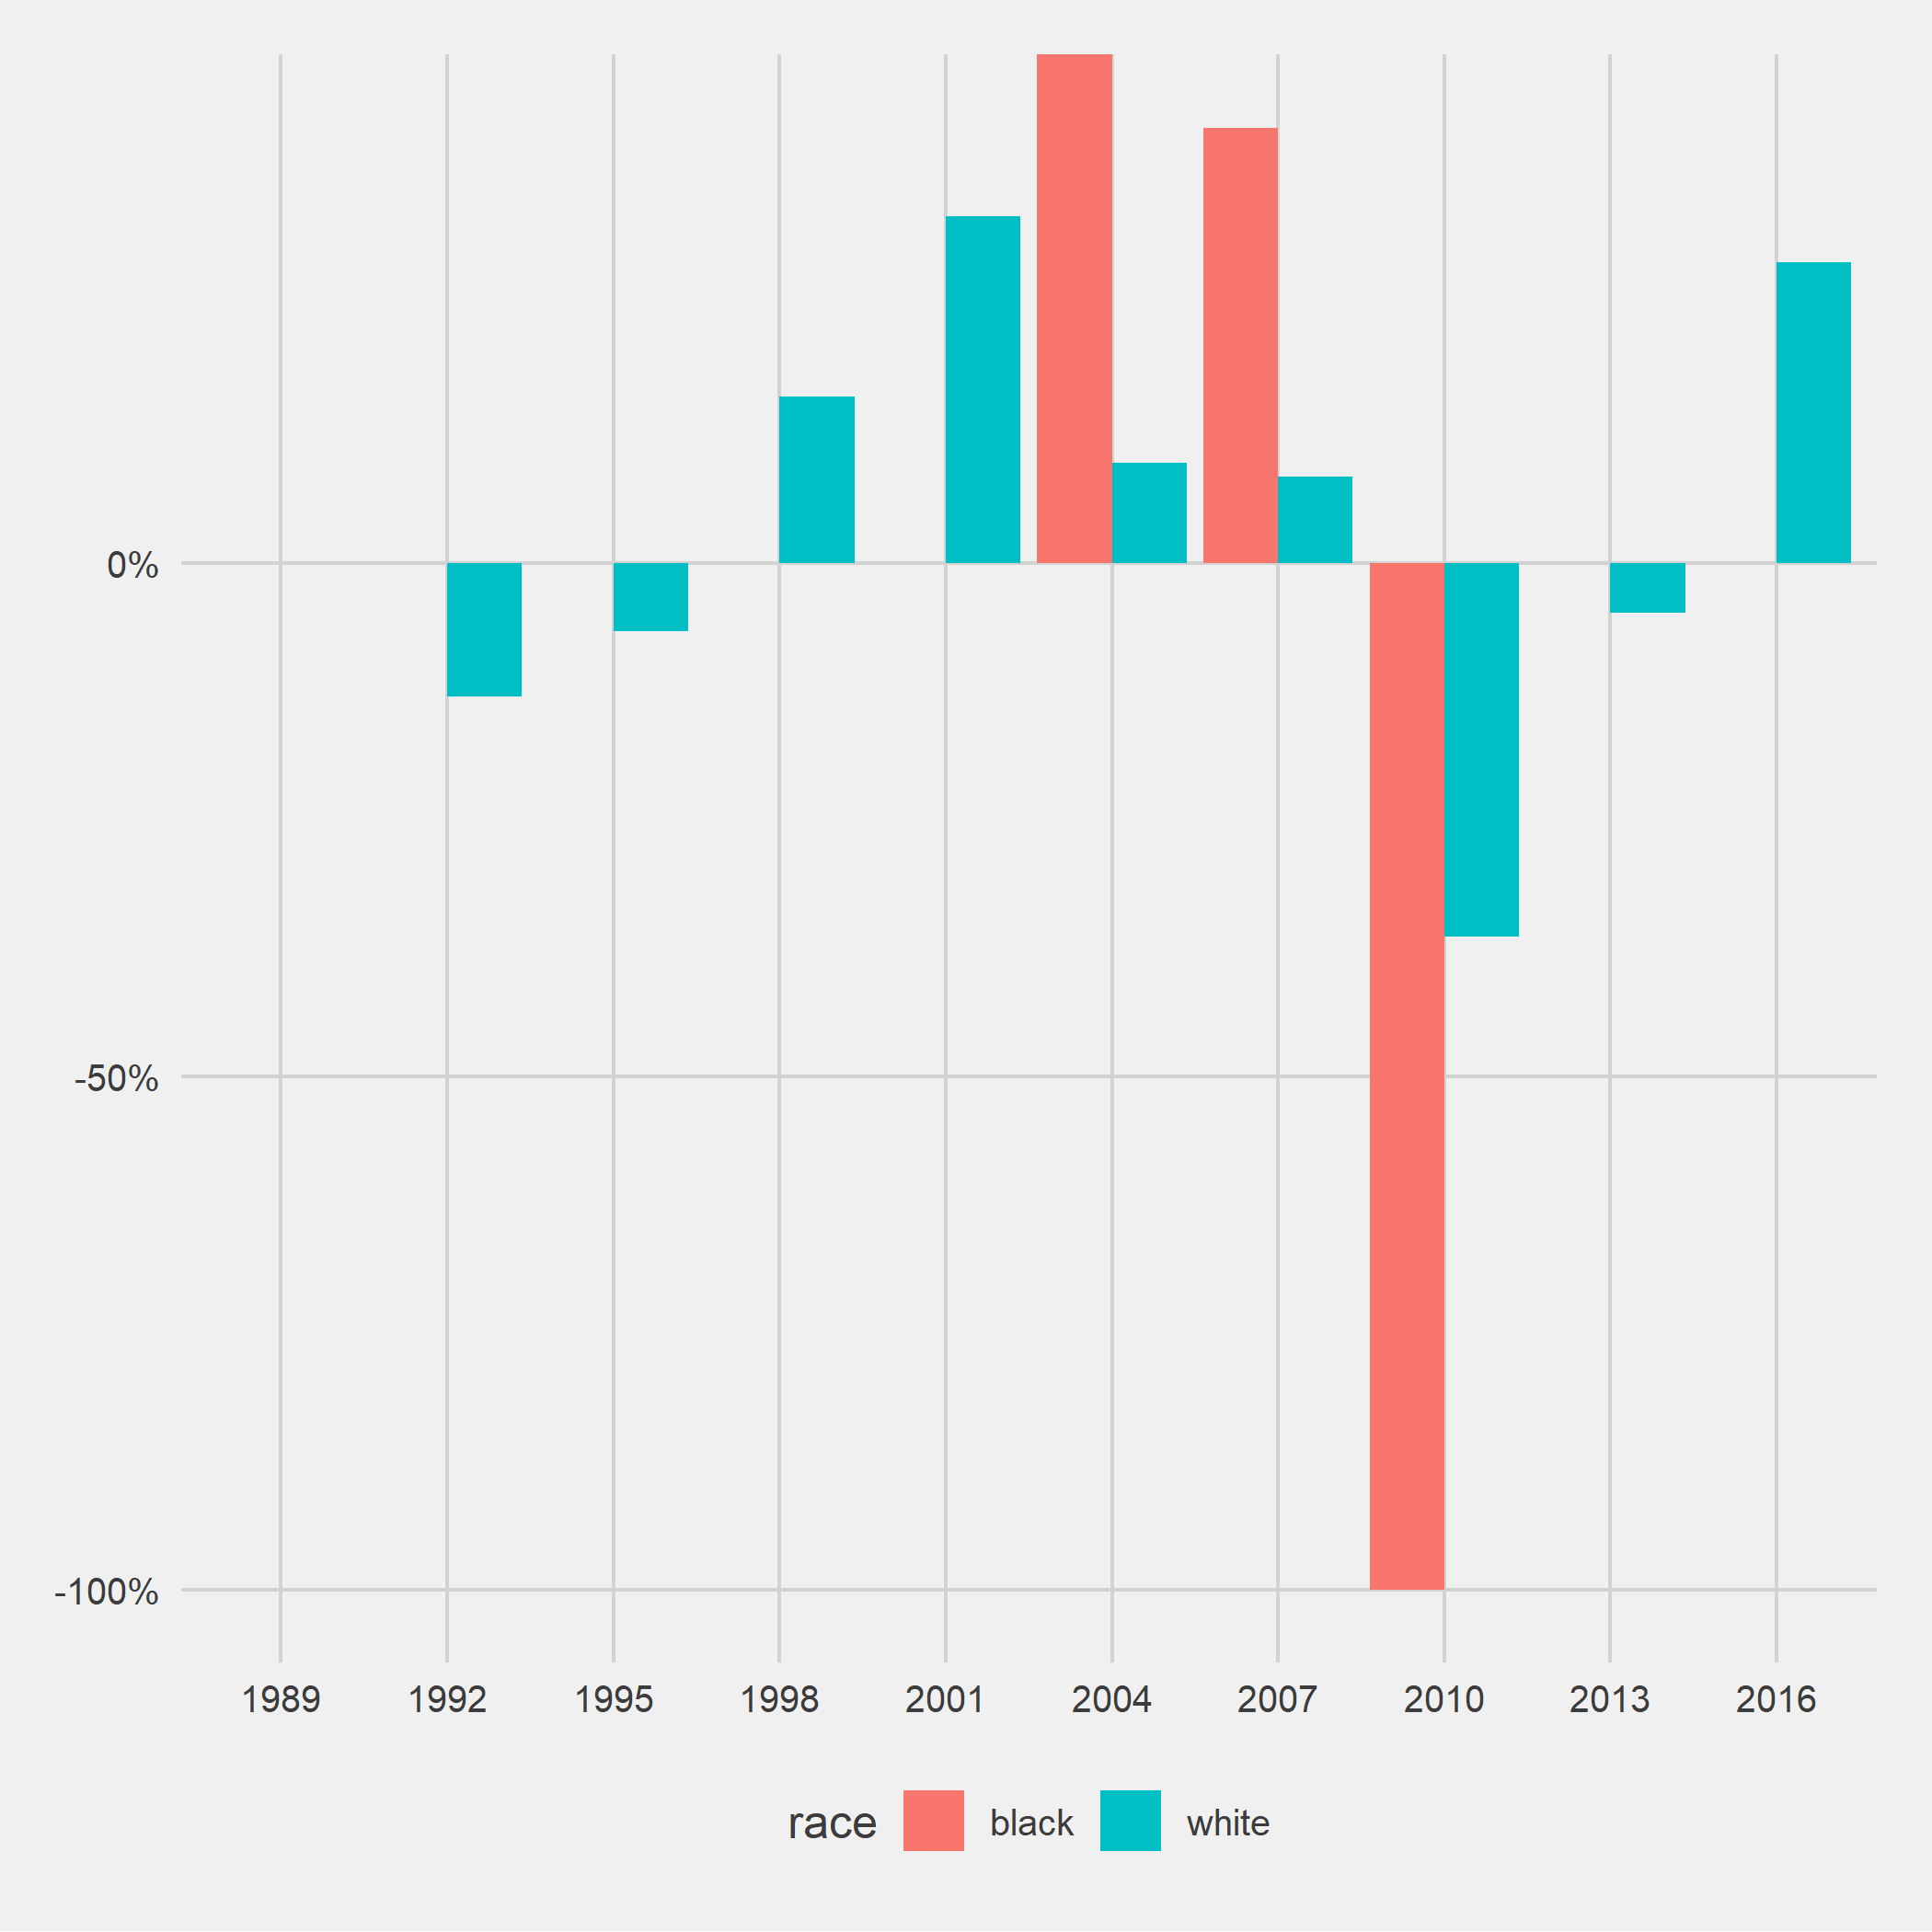
\includegraphics[width=\linewidth, height=5cm]{../change_median hwealth finance_survey_bw_25 _by race .png}
	\end{subfigure}
	\begin{subfigure}{.49\textwidth}
		\centering
		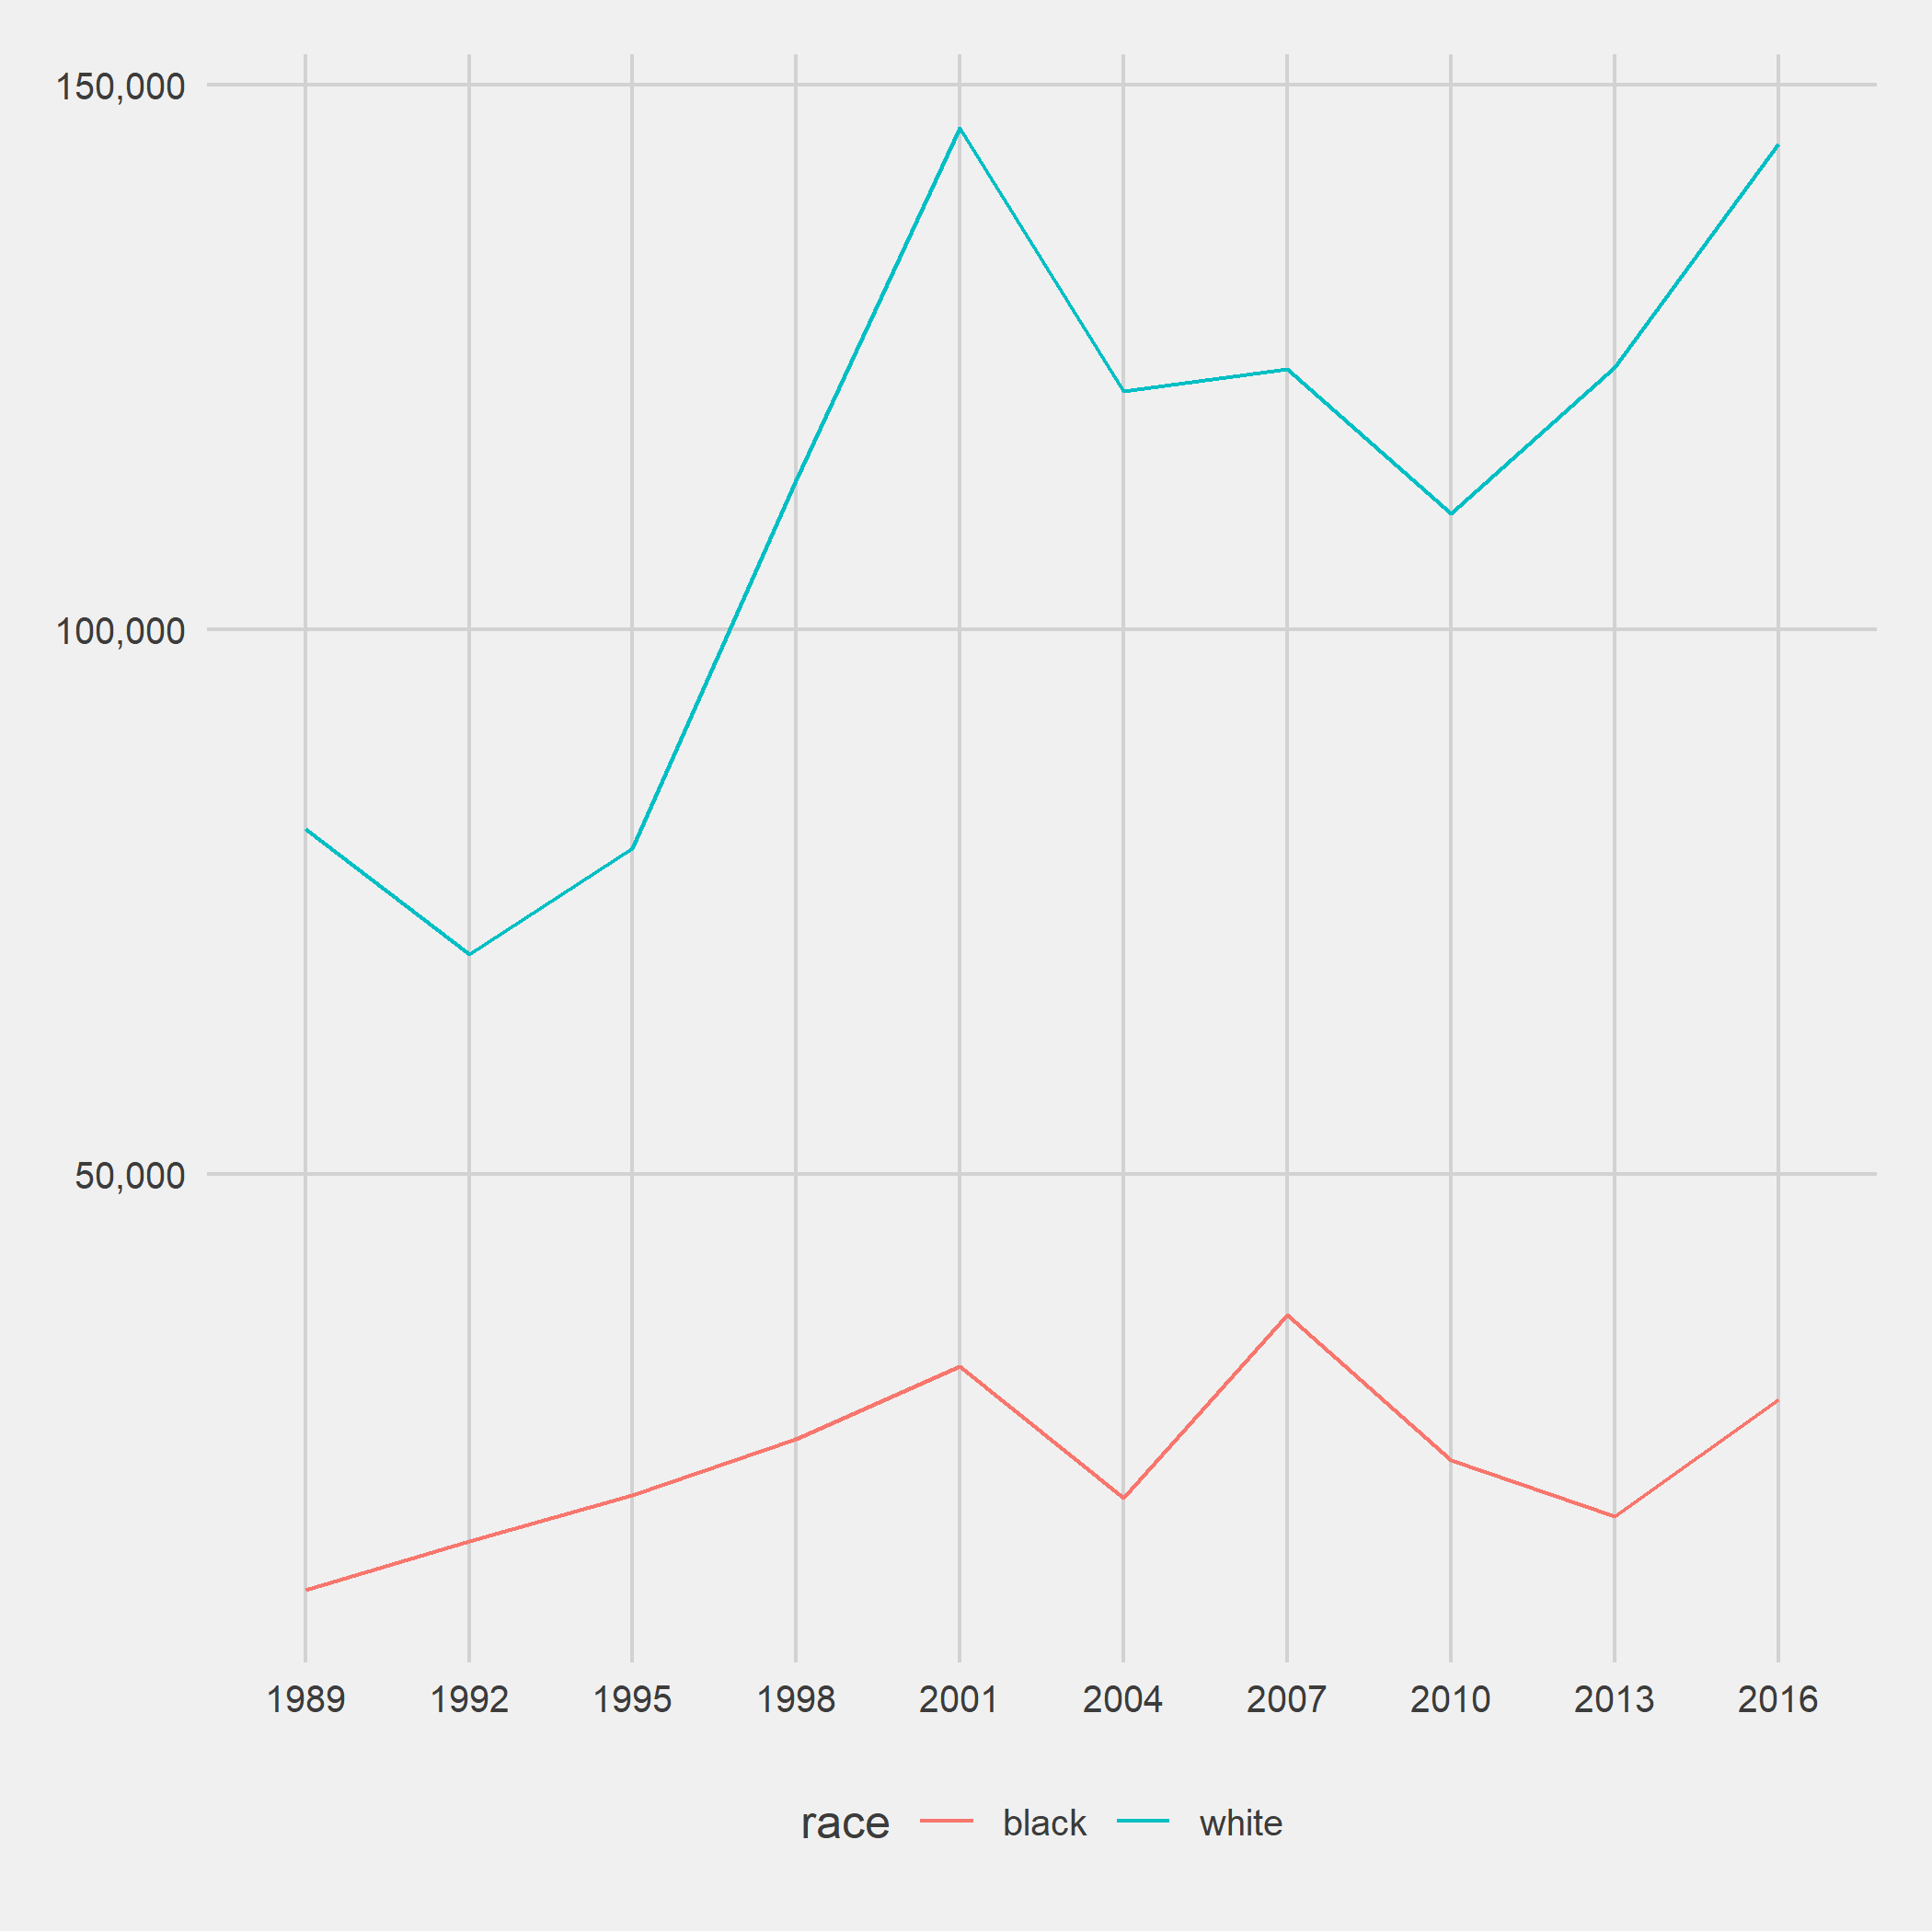
\includegraphics[width=\linewidth, height=5cm]{../median non_hwealth finance_survey_bw_25 _by race .png}
	\end{subfigure}
	\begin{subfigure}{.49\textwidth}
		\centering
		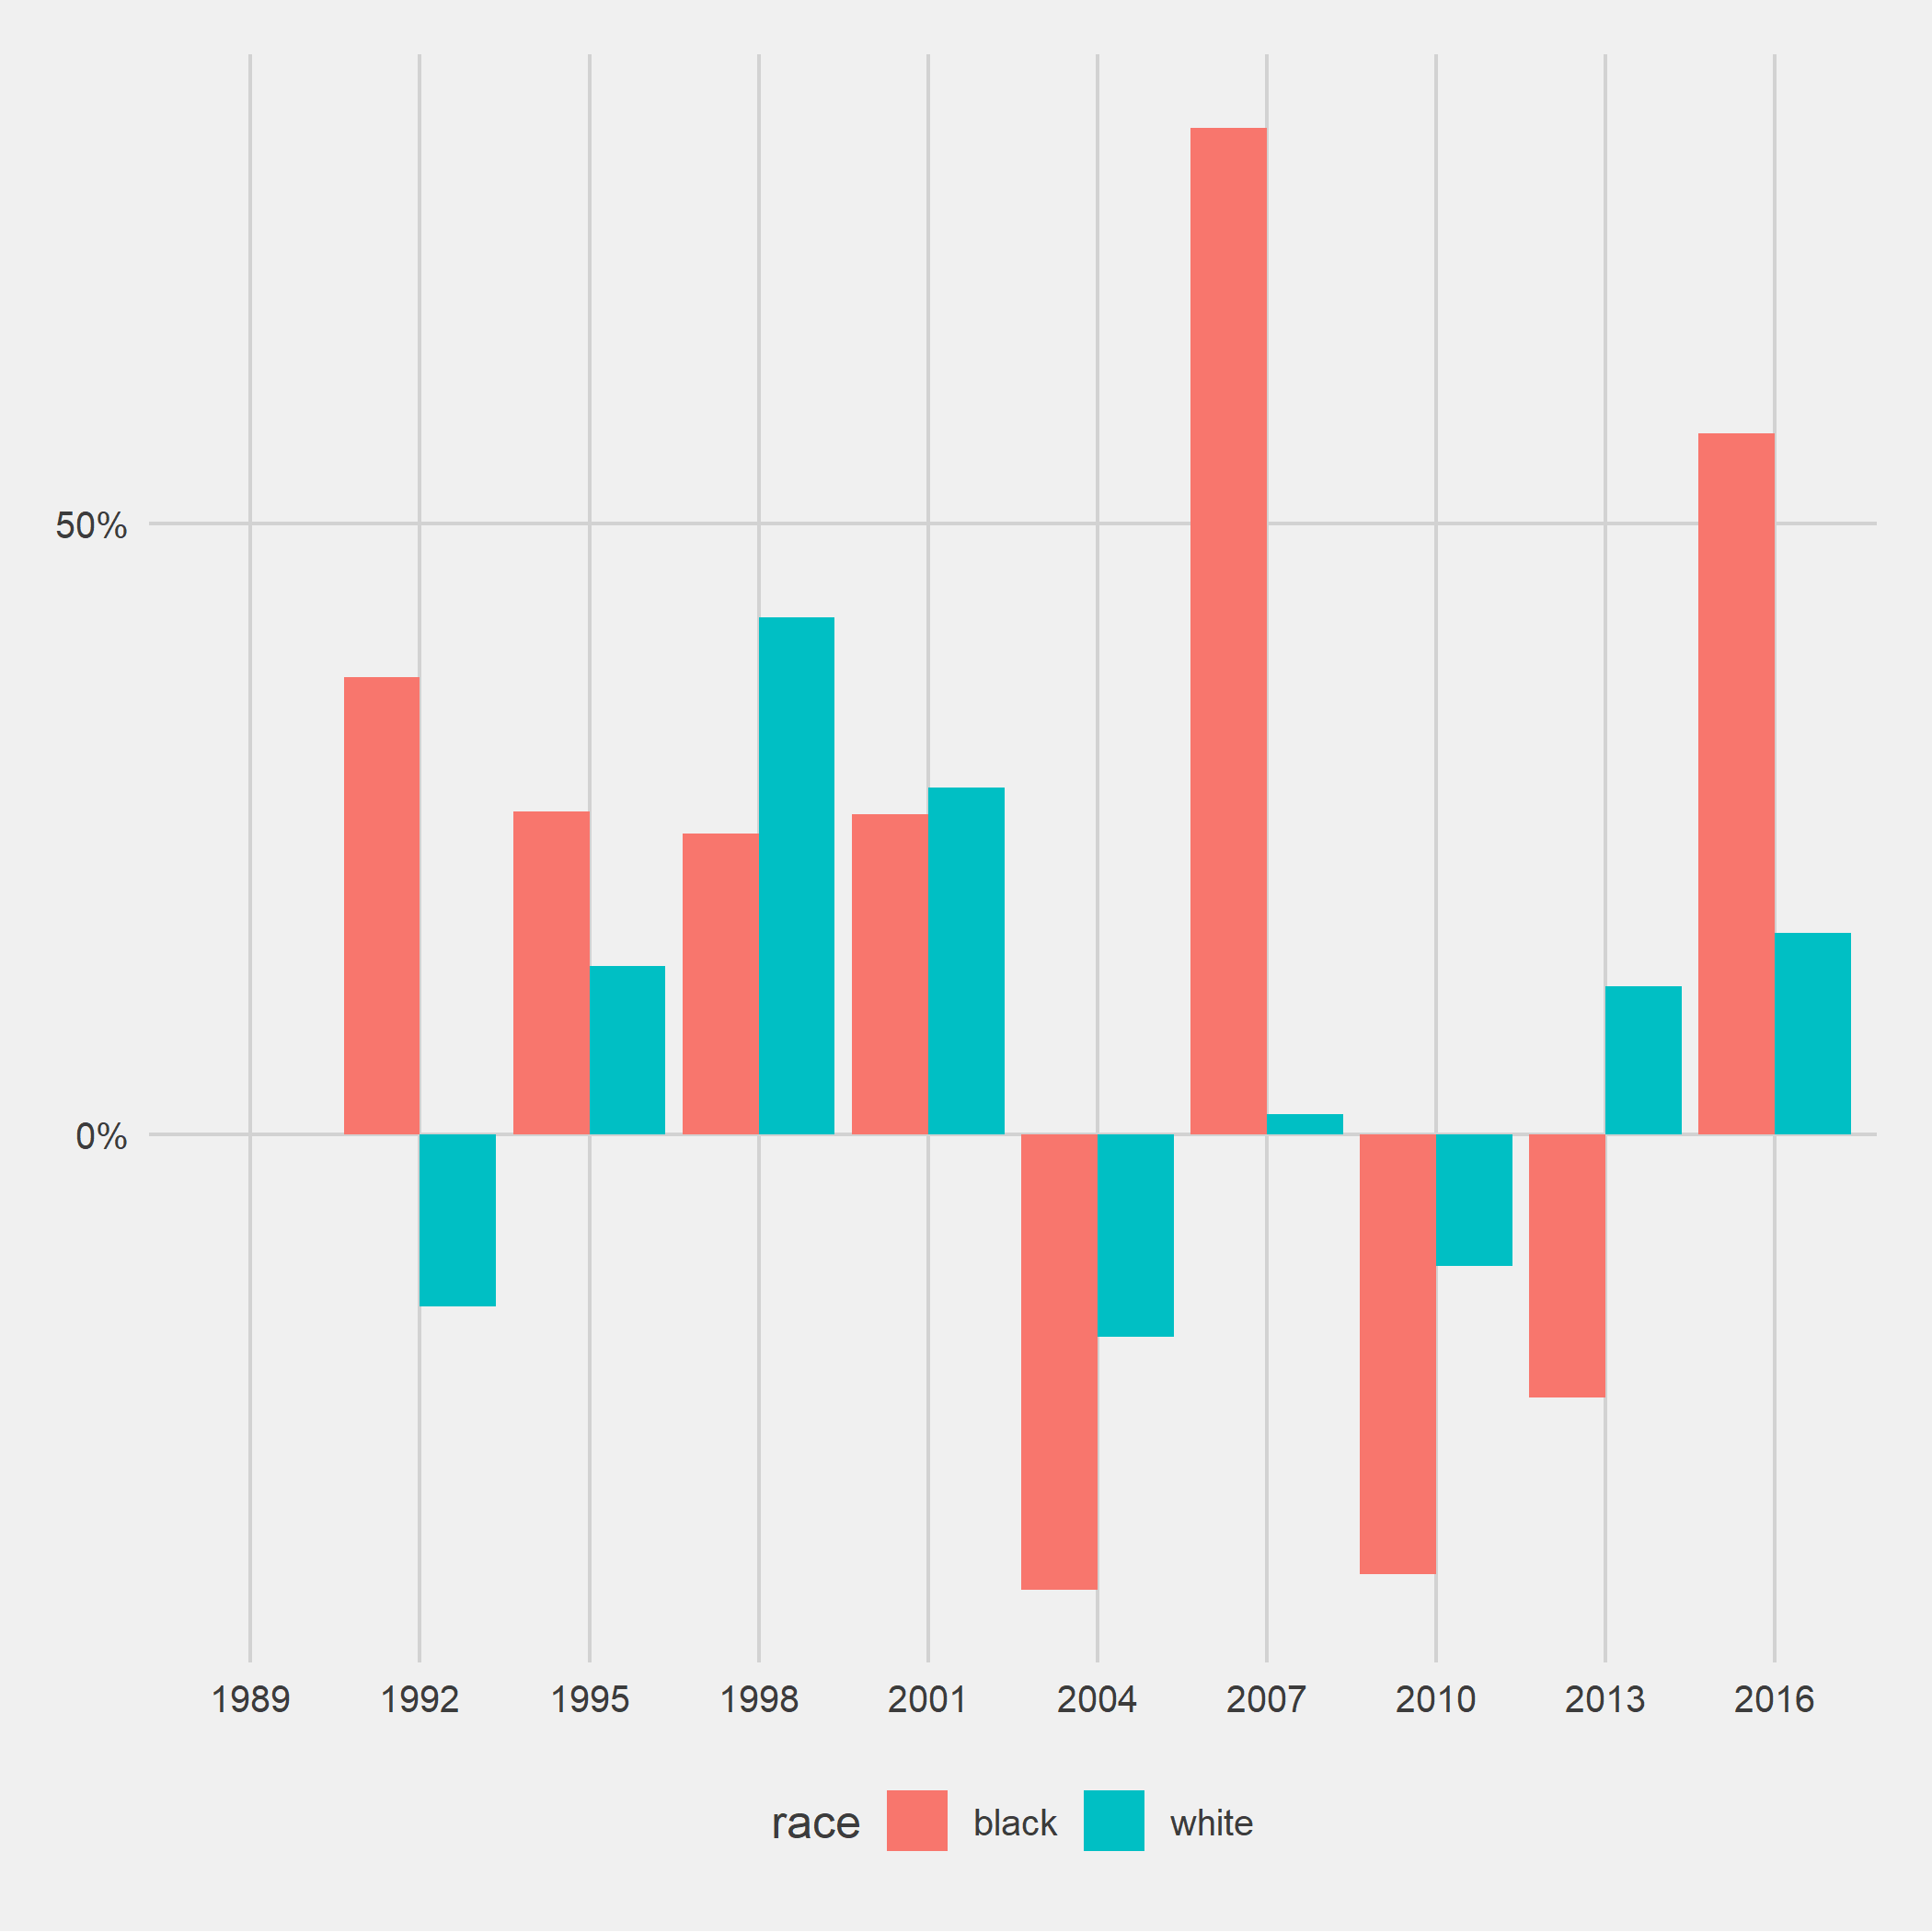
\includegraphics[width=\linewidth, height=5cm]{../change_median non_hwealth finance_survey_bw_25 _by race .png}
	\end{subfigure}
	\caption{Median wealth in 2016 \$ over time by race and level of education}\label{fig:bw25_htrends}
\end{figure}
\begin{table}[h]
	\centering
	\caption{Housing Wealth Losses per Race}
	\label{key}
	\begin{tabular}{@{\extracolsep{5pt}} lcc}
		\\[-1.8ex]\hline
		\hline \\[-1.8ex]
		&	Median Loss	&	Median Percentage Loss\\ \hline
		\bfseries{Three Years after 2007} \\
		Black	&	-14.214\$	& -20.5\% \\
		White	&	-36,955\$& -28.0\% \\
		\bfseries{Nine Years after 2007} & & \\
		Black	&	-9,481\$ & -13.6\%\\
		White	&	-20,014\$ & -15.2\% \\
		\hline \\[-1.8ex]
	\end{tabular}
\end{table}

\subsection*{Question 4}
\textit{Many potential channels have been identified for explaining the wealth gaps by race documented in
	question 1. These include differences in access to financial markets, segregation, discrimination, family
	networks, neighborhood characteristics, and barriers to human capital accumulation. Please pick at
	least two hypotheses (they do not need to be included in the list above) and explain what evidence you
	might want to assemble to test the importance of these channels.} \\



\end{document}
